\documentclass[%
  a4paper,%
  oneside,
  nexus,
  11pt,% <10pt, 9pt>
  %style=screen,
  %sender=bottom,
  blue,% <orange, green, violet>
  %rgb, <cmyk>
  %mono,
  %extramargin,
  %marginleft, <marginright>
  ]{tubsreprt}

\usepackage[utf8x]{inputenc}
\usepackage[ngerman,english]{babel}
\usepackage[numbers]{natbib}
\usepackage{spverbatim}
\usepackage{fancyvrb}
\usepackage{fvextra}
\usepackage{listings}
\usepackage{float}
\usepackage{color}
\usepackage{graphicx}
\usepackage{amsmath}                    % Packages für Formeln
\usepackage{amsthm}			% -||-
\usepackage{amsfonts}			% -||-
\usepackage{amssymb}			% -||-
\usepackage{lscape}			% Querformatiges Beschreiben einzelner Abschnitte mit \begin{landscape} Text \end{landscape}

\usepackage{tikz} 			% TikZ - ein geniales Zeichentool vor allem für Skizzen oder Schemata, Programmabläufe, etc.
\usepackage{pgf}			% Für Tikz
\usepackage{pgfplots} 			% Plots mit TikZ
\usetikzlibrary{shapes,backgrounds, arrows, positioning, trees, shadows}	% Bibliotheken für Tikz
\usepackage{pgfgantt}			% Zum Erstellen eines Gantt-Charts

\graphicspath{{./graphics/}}

%===============================================================
%
%	Hyperlinks im Dokument
%
%---------------------------------------
\definecolor{dkgreen}{rgb}{0,0.6,0}
\definecolor{gray}{rgb}{0.5,0.5,0.5}
\definecolor{mauve}{rgb}{0.58,0,0.82}

\lstset{frame=tb,
  language=Java,
  aboveskip=3mm,
  belowskip=3mm,
  showstringspaces=false,
  columns=flexible,
  basicstyle={\small\ttfamily},
  numbers=none,
  numberstyle=\tiny\color{gray},
  keywordstyle=\color{blue},
  commentstyle=\color{dkgreen},
  stringstyle=\color{mauve},
  breaklines=true,
  breakatwhitespace=true,
  tabsize=3
}

\usepackage[
  pdftex,%
  hidelinks,%
  linktocpage, breaklinks
]{hyperref}				% Package für Lesezeichen und Verlinkungen

%===============================================================
%
%	Glossary
%
%---------------------------------------

\usepackage[nonumberlist,acronym,section]{glossaries}
	%nonumberlist: no page numbering
	%acronym: abbreviations list
	%toc: entry in table of contents
	%section: in toc placed at section level
	%nopostdot: no dots after description
				
\newglossary[slg1]{symbolslist}{syi}{syg}{List of Symbols}			% symbols
\newglossary[alg]{acronymlist}{acr}{acn}{List of Abbreviations}			% abbreviations	

\makeglossaries

\AtEndDocument{\glsaddall}	%füge alle Symbole dem Verzeichnis zu

%-----------------------------------------------------------------


%Makros für eine erleichterte Eingabe wiederkehrender Befehle:
\addto\captionsngerman{
  \renewcommand{\figurename}{Figure}
}
\newcommand{\abb}[1]{Figure~\ref{#1}}
\newcommand{\tab}[1]{Tabelle~\ref{#1}}
\newcommand{\glg}[1]{Gleichung~\ref{#1}}
\newcommand{\kap}[1]{Kapitel~\ref{#1}}
\newcommand{\abschn}[1]{Abschnitt~\ref{#1}}
\newcommand{\anh}[1]{Anhang~\ref{#1}}

\newcommand{\ul}{\underline}
\newcommand{\ol}{\overline}
\newcommand{\tb}{\textbf}
\newcommand{\ts}{\textsl}

\newcommand{\kalman}{\textsc{Kalman}-Filter }

%===============================================================
%
% Farben
%
%-------------------------------

\definecolor{ilr-blue}{RGB}{44,79,162}
\definecolor{light-blue}{RGB}{220,220,255}
\definecolor{gray90}{gray}{0.9}
\definecolor{gray80}{gray}{0.8}
\definecolor{gray60}{gray}{0.6}
\definecolor{gray50}{gray}{0.5}
\definecolor{gray40}{gray}{0.4}
\definecolor{gray20}{gray}{0.2}

%===============================================================
%
% Titelseiten-Elemente
%
%-------------------------------

\title{\LARGE R 2336 S  \newline Analysis of Tasking Algorithms for efficiently operating Sensor Networks} \subtitle{Institute of Space Systems}
\author{Vipul Dilip Solanke}

%---------------------------------------------------------------

\logo{
\includegraphics{iraslogo_englisch.png}} % ilrlogo_englisch.png
\titlepicture{doctor_pop2009.jpg}

%===============================================================
%
% Hurenkinder/Schusterjungen vermeiden
%
\clubpenalty         = 10000
\widowpenalty        = 10000
\displaywidowpenalty = 10000

%---------------------------------------------------------------------------------------------------


\begin{document}

  \maketitle[image] %[<plain/image/imagetext>,<logo=left/right>]

  \chapter*{Aufgabenstellung}

Die Originalaufgabenstellung ist bei Studienarbeiten dem ungebundenen Institutsexemplar beizufügen, bei Bachelor-, Master- und Diplomarbeiten dem 
gebundenen Exemplar zur Vorlage bei der Fakultät. Die Aufgabenstellung bei Bachelor-, Master- und Diplomarbeiten wird vom Fachbereich ausgegeben 
(bei CSE-Masterarbeit vom CSE Office), dieser registriert den Beginn und die Abgabe der Arbeit und stempelt diese Angaben auf das letzte Blatt der 
Original-Aufgabenstellung.

Eine Diplom-, Studien-, Bachelor- bzw. Masterarbeit soll zeigen, dass man in der Lage ist, in begrenzter Frist eine Aufgabe nach wissenschaftlichen Methoden 
selbständig zu bearbeiten.

Die Aufgabenstellung kann Literaturhinweise enthalten, die als Einstieg in die Aufgabe gedacht
sind. Es wird erwartet, daß weitere Literatur selbständig gesammelt wird (Bibliotheken
der TU, des Instituts, etc.).

\tb{Wichtig:} Schriftverkehr mit Dritten bei Nennung des die Arbeit betreuenden Instituts bedarf der
vorherigen Genehmigung.
\\ 
\\
In der Abgabeversion dann dieses Blatt entfernen und an dieser Stelle durch die Aufgabenstellung ersetzen!

  \chapter*{Declaration in lieu of an oath}

I hereby declare in lieu of an oath that I have written the following thesis independently and only with the
with the aid of the literature indicated.

\vspace{2cm}
\tikz\draw (0,0) -- (7,0);

Date, Signature

  \chapter*{Abstract}

The number of artificial objects in the near-Earth space realm is on a consistent rise each year,
posing a serious threat to the safety of operational space assets. Effective Space Situational Awaren-
ess (SSA) practices are vital to continuously update our understanding of the space environment.
This knowledge is essential for implementing appropriate measures to mitigate risks in densely
populated orbits and to enhance sustainability in the near-space domain. In order to mitigate these
risks, continuous monitoring of the space region and building space debris object catalogs is
necessary. To ensure the high accuracy of catalogued objects, the follow-up observations consisting
orbit improvement information are needed. Given the constraints of observation resources, espe-
cially for space debris within the geostationary orbit, where observational windows during the night
are restricted, and considering telescope capabilities, effective sensor tasking of the available sensor network
holds significant importance.\\

This thesis delves into the examination of global sensor networks for space debris observations. It integrates various weighting schemes into the cost function of 
the Greedy algorithm, a tool employed for surveying in the SNS software. The research introduces the application of a genetic algorithm to optimize follow-up observation 
scheduling within a telescope network, with a focal point on catalog maintenance. The primary optimization parameter is the information content associated with the orbit. 
Emphasis is placed on the significance of utilizing orbit covariance and quantifying information gain for effective optimization.
The study concludes with simulations conducted in the Sensor Network Simulator (SNS), a tool suite developed to meticulously study and optimize the performance of existing sensors and their configurations. The effectiveness of the algorithm is analyzed within this framework.

\pagebreak

\chapter*{Kurzfassung}

Die Zahl der künstlichen Objekte im erdnahen Weltraum nimmt jedes Jahr zu,
Sie stellen eine ernsthafte Bedrohung für die Sicherheit der operativen Weltraumressourcen dar. Effektive SSA ist unerlässlich, um unser Verständnis der Weltraumumgebung ständig zu aktualisieren.
Dieses Wissen ist entscheidend für die Umsetzung geeigneter Maßnahmen zur Risikominderung in dicht besiedelten
dicht besiedelten Orbits und zur Verbesserung der Nachhaltigkeit im Nahbereich des Weltraums. Um diese Risiken zu mindern
Risiken zu mindern, ist eine kontinuierliche Überwachung des Weltraums und die Erstellung von Katalogen von Weltraummüllobjekten
notwendig. Um die hohe Genauigkeit der katalogisierten Objekte zu gewährleisten, sind Folgebeobachtungen, die
Informationen zur Verbesserung der Umlaufbahn benötigt werden. Angesichts der begrenzten Beobachtungsressourcen, insbesondere
insbesondere für Weltraummüll in der geostationären Umlaufbahn, wo die Beobachtungsfenster während der Nacht
und unter Berücksichtigung der Teleskopkapazitäten ist eine effektive Nutzung des verfügbaren Sensornetzes
von großer Bedeutung.\\

Diese Arbeit befasst sich mit der Untersuchung globaler Sensornetzwerke zur Beobachtung von Weltraummüll. Sie integriert verschiedene Gewichtungsschemata in die Kostenfunktion des 
des Greedy-Algorithmus, der in der SNS-Software zur Vermessung eingesetzt wird. Die Forschung stellt die Anwendung eines genetischen Algorithmus zur Optimierung der Nachbeobachtung 
Beobachtungsplanung innerhalb eines Teleskopnetzwerks, wobei der Schwerpunkt auf der Katalogpflege liegt. Der primäre Optimierungsparameter ist der mit der Umlaufbahn verbundene Informationsgehalt. 
Der Schwerpunkt liegt auf der Bedeutung der Nutzung der Orbit-Kovarianz und der Quantifizierung des Informationsgewinns für eine effektive Optimierung.
Die Studie schließt mit Simulationen, die mit dem Sensor Network Simulator (SNS) durchgeführt wurden, einem Toolpaket, das entwickelt wurde, um die Leistung bestehender Sensoren und ihrer Konfigurationen genau zu untersuchen und zu optimieren. Die Effektivität des Algorithmus wird in diesem Rahmen analysiert.
  \tableofcontents
  \newpage
   \glossarystyle{altlong4col}%
    \setlength{\glsdescwidth}{0.7\textwidth}
  %----------------------------------------------
%
% Symbolverzeichnis
%
%-----------------------------------------------


% LATIN (use prefix 'x' in sort)
%-----------------------

\newglossaryentry{symb:c} {name=\ensuremath{c},    description={Lichtgeschwindigkeit im Vakuum, \ensuremath{c=299.792.458\; \frac{m}{s}}}, 
symbol=\ensuremath{\frac{m}{s}},       sort=xc,type=symbolslist}
\newglossaryentry{symb:g} {name=\ensuremath{g},    description={Erdbeschleunigung}, symbol=\ensuremath{\frac{m}{s^{2}}},       sort=xg,type=symbolslist}
\newglossaryentry{symb:m} {name=\ensuremath{m},    description={Masse},             symbol=\ensuremath{kg},                    sort=xm,type=symbolslist}
\newglossaryentry{symb:E} {name=\ensuremath{E},    description={Energie},           symbol=\ensuremath{J},                     sort=xE,type=symbolslist}
\newglossaryentry{symb:J2}{name=\ensuremath{J_{2}},description={Koeffizient f\"ur die Abplattung der Erde}, symbol=\ensuremath{},sort=xJ2,type=symbolslist}

% GREEK (use prefix 'y' in sort)
%------------------------

\newglossaryentry{symb:OmegaE}{name=\ensuremath{\Omega_{E}},description={Winkelgeschwindigkeit der Erde}, symbol=\ensuremath{\frac{rad}{s}}, 
sort=yOmegaE, type=symbolslist}
\newglossaryentry{symb:rho}{name=\ensuremath{\rho}, description={Dichte}, symbol=\ensuremath{kg/m^{3}}, sort=yrho, type=symbolslist}

% INDICES (use prefix 'z' in sort)
%-------------------------
\newglossaryentry{Index:min}{name=\ensuremath{min},description={Minimalwert},symbol=\ensuremath{}, sort=zmin, type=symbolslist}
\newglossaryentry{Index:max}{name=\ensuremath{max},description={Maximalwert},symbol=\ensuremath{}, sort=zmax, type=symbolslist}
  %----------------------------------------------
%
% Abkürzungsverzeichnis
%
%-----------------------------------------------

\newacronym{DLR}{DLR}{Deutsches Zentrum f\"ur Luft- und Raumfahrt}
\newacronym{ILR}{ILR}{Institut f\"ur Luft- und Raumfahrtsysteme}
\newacronym{ERIG}{ERIG}{ExperimentalRaumfahrt - InteressenGemeinschaft e.V.}
\newacronym{STERN}{\textsc{STERN}}{Studentische Experimentalraketen} 
  
  \chapter{Einleitung}

Die Einleitung soll einen Überblick über den Stand der Technik geben, das zu unter-
suchende System beschreiben und die Aufgabenstellung mit eigenen Worten näher
erläutern.

\section{Ziele der Arbeit}

\section{Vorgehensweise}

Hier wiedergeben, wie die zuvor definierten Ziele in den folgenden Kapiteln umgesetzt werden, etwa:

In \kap{sec:grundlagen} werden die theoretischen Grundlagen behandelt, wonach dann in \kap{sec:hauptteil} die Software-Architektur festgelegt und 
beschrieben wird.
  \chapter{Theoretical principles}
\label{sec:grundlagen}

This study builds upon prior research in several key areas. To facilitate comprehension, it commences with an exploration of fundamental principles in orbital mechanics. As the main focus of the thesis is upon geostationary orbit,
it's primary uses, benefits and potential  threats are described.
Subsequently, it provides an introduction to SSA and offers an overview of global SSA sensor networks. Lastly, it presents research findings
 related to sensor tasking.

\section{Background}
Satellites play a crucial role in supporting a wide range of applications and services. However, the presence of uncontrolled defunct satellites, spent rocket stages, 
and other space debris in Earth's orbital pathways poses a significant risk to operational satellites. This debris results from various factors, including explosions, 
collisions, and even intentional practices such as leaving discarded rocket stages or releasing covers and materials after deploying a satellite into its designated orbit.\\

Earth's orbital realm is neatly categorized into various types, with the most prevalent ones being Low-Earth Orbit (LEO), Medium-Earth Orbit (MEO), and the esteemed Geostationary-Earth Orbit (GEO).
Each orbit type boasts its own unique attributes, making it the ideal choice for specific applications. Therefore, monitoring diverse domains requires distinct sensors and surveillance techniques. 
While radar technology is effective for lower orbits, the considerably higher geostationary orbit necessitates the utilization of "deep space radars." However, the use of these radars is constrained 
by the limited number of systems available worldwide. As a result, higher orbits demand the keen eyes of optical telescopes for observation. However, optical observations come with their own set of complexities, 
including the absence of distance information and vulnerability to adverse viewing conditions. It is precisely these intricate challenges that drive the core motivation of this research – the 
specialized endeavor of correlating optical observations to derive a comprehensive orbital solution.


\section{Space Situational Awareness}

With ever so increasing space activities, it is of utmost importance to ensure the safety of these space assets. As already described, there are thousands and thousands of
space debris objects, which can prove to be potential threats to current functional satellites and future launches. SSA is the thorough understanding
of the orbits, tracking and identifying the objects and the prediction of their future positions to ensure safe space and avoiding future collisions.





\subsection{components of SSA}
\begin{itemize}
  \item Object Catalogs : The object catalogues are the foundation of the SSA. These object catalogues contain information about functional and non functional satellites, the residual rocket body parts and the space debris objects that are originated from the collision of RSOs. The object catalogues contain valuable information such as origin, size of the objects, orbit information and other necessary details \cite{esa6}.
  \item Tracking Systems : To build above mentioned catalog and to monitor the objects, SSA uses the various sensor networks, such as ground-based networks (RADAR, Optical telescopes) and space-based (in-situ) sensors. The data acquired from these networks is then interpreted to calculate positions, velocities and to determine orbits of these objects \cite{esa6}.
  \item Orbital Analysis and Predictions : This is the important aspect of SSA which takes the data from sensor networks and with the help of available orbit determination and propagation tools, predict the future positions and velocities of the space debris objects. This information helps to analyze the possible close encounters or conjunction other objects, and thereby preventing catastrophic collisions with suitable protective measures \cite{esa6}.
  \item Conjunction alerts and notifications : The SSA systems are well equipped to provide warnings and alerts in case two objects are in close proximity and there are chances of collision. The operators are informed and alerted about such events so that protective measures can be taken in well advance \cite{esa6}.
  \item Space Weather Monitoring : In addition to space debris monitoring, SSA systems also help in monitoring space weather conditions. The timely updates regarding cosmic radiations and solar flares can be useful in planning satellite operations and rendezvous activities \cite{esa6}.
\end{itemize}

\subsection{Types of sensors}

\subsubsection{RADAR}

Radar, an abbreviation for Radio Detection and Ranging, stands out as a valuable sensor for observational purposes and plays a crucial role in the foundation of SSA. It can be divided into primary and secondary systems. Primary systems rely solely on the reflected radiation from the observed object, while secondary systems involve an active response signal from the object. When monitoring passive objects, primary systems are typically considered. Radar finds widespread application in various observations, 
such as spotting aircraft, enforcing speed limits for motor vehicles, and determining weather conditions. These systems can be ground-based, portable as handheld devices, or mounted on aircraft. One notable advantage of radar over telescopes is its capacity to detect objects independently of light. Additionally, radar's use of electromagnetic waves is less 
affected by environmental factors like fog, rain, or snow compared to telescopes \cite{weeden}.\\

Typically comprised of at least one transmitter and receiver, radars emit radio waves at specific frequencies. The reflected waves, upon encountering a target, are measured by the receiver, enabling the calculation of the target's location in relation to the radar. Radars offer the distinct advantages of actively measuring both the range and range rate to a target, with certain types capable of concurrently tracking multiple objects. However, these merits are offset by significant drawbacks, including high costs associated with initial construction, operations, and maintenance, as well as considerations of size and complexity \cite{weeden}.\\

In the nascent stages of space exploration, two radar concepts emerged for tracking space objects. The first concept involved interferometer-based systems, also known as bi-static or multi-static systems, as seen in Figure~\ref{fig:bistatic}, where the receiver and transmitter(s) were strategically separated by a specific distance. Particularly suitable for ''fence'' applications, these bistatic radar systems emit a continuous stream of energy in a specific direction, effectively tracking any object passing through the designated "radar fence" \cite{bistat}. A typical example of such RADAR is ''Space Fence'' radar facility in Marshall Islands, USA developed by Lockheed Martin. The Space Fence, 
currently the most sophisticated radar globally, offers unanticipated detection, tracking, and precise measurement of space objects, such as satellites and orbital debris, mainly in LEO \cite{fence}.\\

\begin{figure}[H]
	\centering
	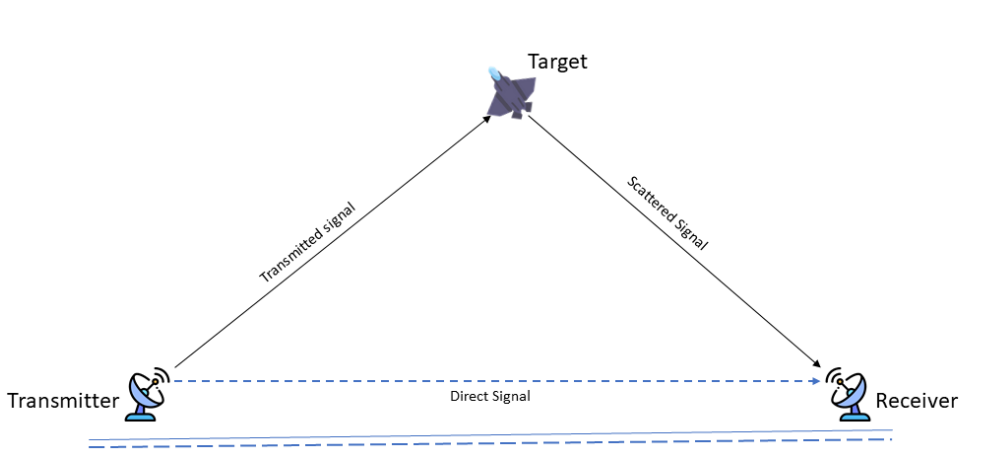
\includegraphics[width=0.95\textwidth]{bistatic.png}
	\caption{ Bi-static system of the RADAR, inspired by \cite{bistat}}\label{fig:bistatic}
\end{figure}

The second initial radar concept was the monostatic radar, the general working principle of monostatic radar as seen in Figure~\ref{fig:monostat}, featuring collocated transmitting and receiving antennas typically mounted on a rotatable and elevatable parabolic dish. Referred to as mechanical trackers, these monostatic radars excel in precision tracking of individual or a small number of objects. With sufficient power, they can extend their tracking capabilities to space objects in the GEO belt, even beyond 36,000 kilometers. In regions with adverse weather conditions, mechanical tracking radars are often housed within domes made of materials transparent to electromagnetic radiation at their operational frequency \cite{weeden}.\\
For such RADAR, Tracking and Imaging Radar (TIRA) is 
a perfect example. The TIRA system, featuring a 34-meter diameter antenna housed in a spherical structure, is a central experimental facility designed for the development and exploration of radar techniques in detecting and reconnoitering space objects. This versatile system, capable of a complete 360° azimuth rotation and 90° elevation movement, weighs 240 tons and achieves a rapid 24° per second rotation in azimuth, completing a full revolution in just 15 seconds. TIRA's dual functionality includes a narrowband, fully coherent, high-power tracking radar operating at L-band (1,333 GHz) and a wideband imaging radar with a transmission frequency in Ku-band (16.7 GHz) that presently features high target resolution. 
Beyond its experimental role, TIRA plays a crucial supporting role in space missions, with space agencies worldwide leveraging the specialized capabilities of Fraunhofer scientists and their cutting-edge radar system \cite{tir}.\\

\begin{figure}[H]
	\centering
	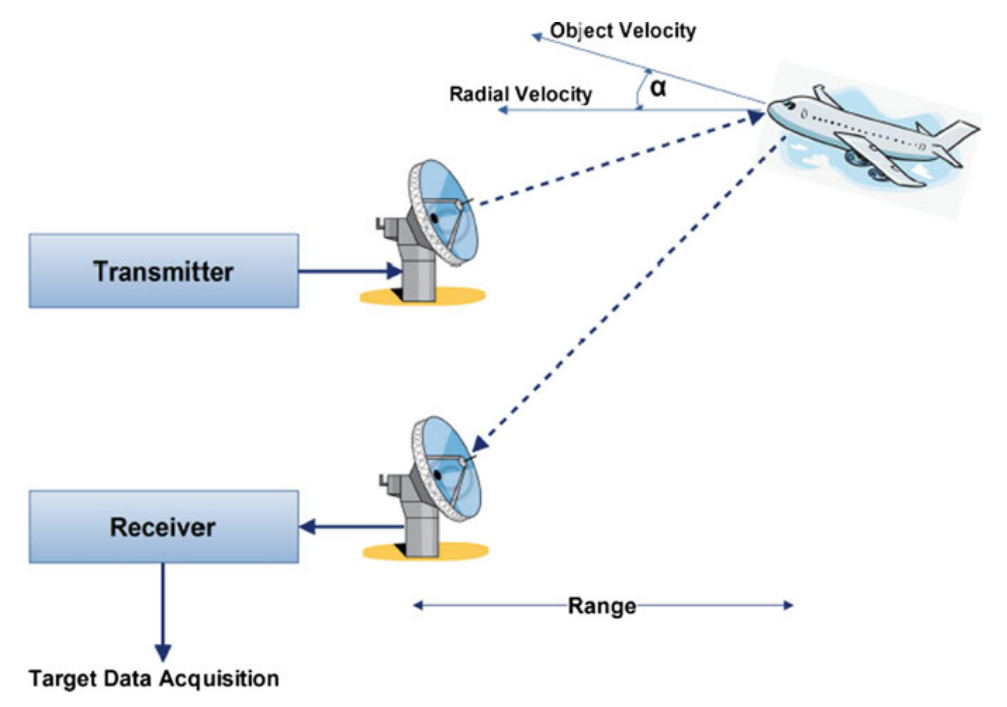
\includegraphics[width=0.7\textwidth]{monostatic.png}
	\caption{ A general principle of the simple monostatic continuous radar system \cite{jena2019}}\label{fig:monostat}
\end{figure}


As the space era progressed, two additional radar paradigms emerged: monostatic and bi-static radars employing phased array antennas, as seen in the Figure~\ref{fig:phased}. Phased arrays consist of small, identical antennas mounted on a fixed face, capable of varying the phases of their signals. This allows the effective radiated energy to be steered or focused in specific directions, with the potential for multiple independent beams of energy to be individually directed towards multiple targets simultaneously. While phased arrays offer enhanced capabilities, they also entail more complex supporting systems compared to mechanical radars \cite{Reed}. An illustrative example is depicted in Figure~\ref{fig:phased}, showcasing a monostatic phased array with two separate faces operated by the U.S. military.

\begin{figure}[h!]
	\centering
	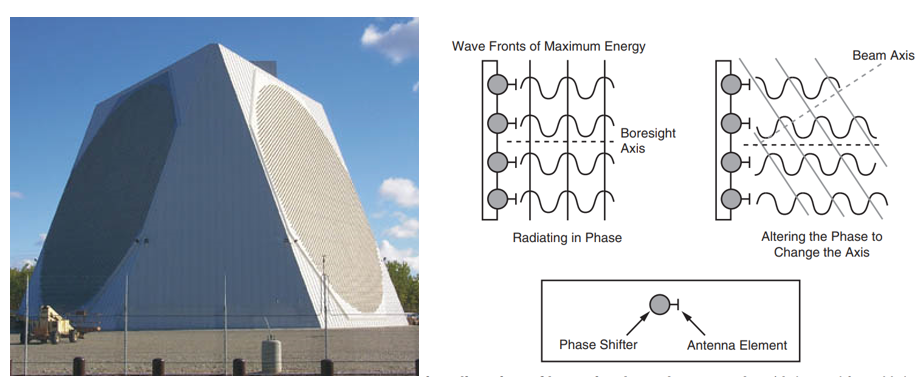
\includegraphics[width=0.9\textwidth]{phase.png}
	\caption{ PAVE PAWS phased array at Clear AFS, Alaska (left) \cite{monostat} and  Changing direction of beam in phased-array radar. (Adapted from University of Wisconsin Naval 
  ROTC, “Naval Weapons Systems Lesson 7: Electronic Scanning and Phased Array Radars,” course files) \cite{usssn}}\label{fig:phased}
\end{figure}

\subsubsection{Optical sensors}

Optical telescopes, as integral components of space object tracking systems, necessitate specific environmental conditions for optimal functionality. In contrast to radar systems, telescopes are passive optical sensors reliant on electromagnetic radiation emitted by celestial bodies. Observations of space debris using telescopes require a dark and nocturnal sky to avoid interference from sunlight during the daytime, which could hinder object detections \cite{optical}. Furthermore, an unobstructed sky, free from cloud cover, is essential for telescope operations.\\

Telescopes face unique considerations concerning external illumination. Unlike lasers, telescopes do not emit their own light radiation; instead, they depend on sunlight to illuminate space objects. Consequently, objects within Earth's shadow may be challenging to detect. However, for LEO objects there is a time window after sunset and before sunrise when the sun is below the horizon, but objects are still illuminated by sunlight and observed effectively \cite{optical}. The reflective properties of an object's surface material further influence the quality of observations, introducing considerations of reflection and absorption \cite{optical}.\\

\begin{figure}[h!]
	\centering
	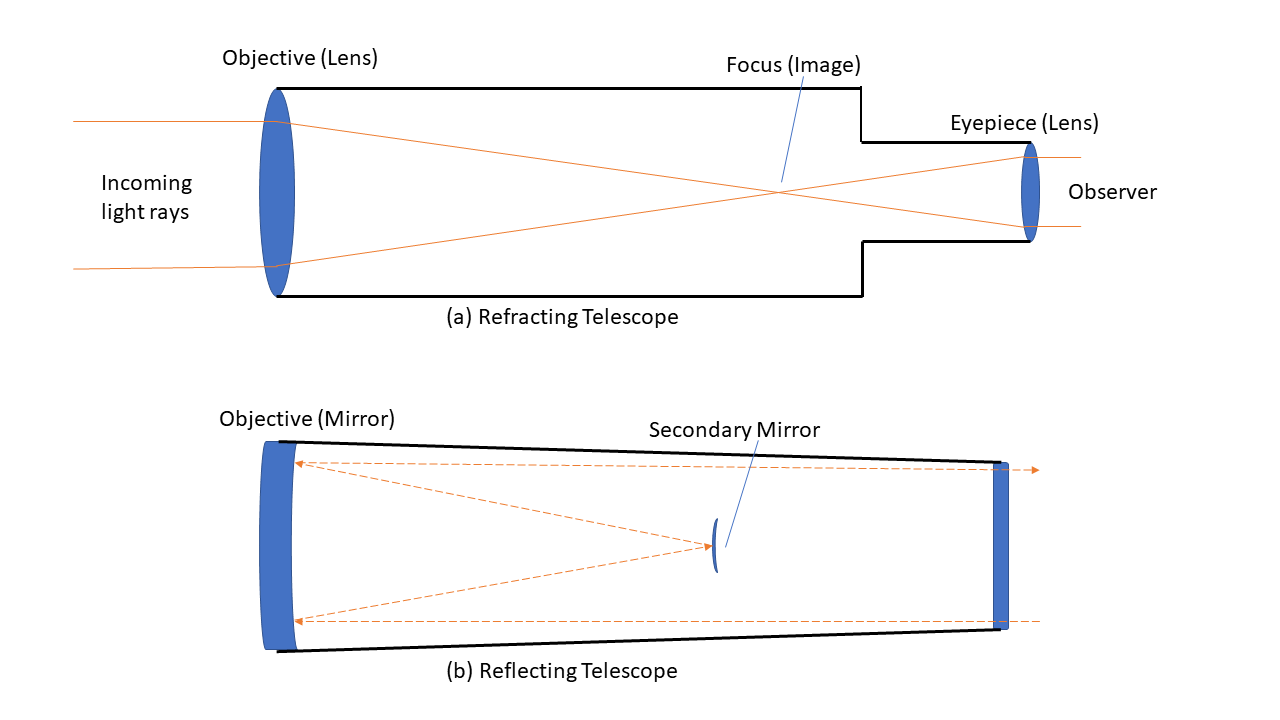
\includegraphics[width=0.9\textwidth]{lens.png}
	\caption{Refracting and Reflector Telescope, inspired by \cite{tele}}\label{fig:lensopt}
\end{figure}

The aperture, denoting the diameter of the light-collecting region, is a crucial parameter for telescopes \cite{astro}. Two primary categories of telescopes, refracting and reflecting, differ in their approaches to light collection. Refracting telescopes use a converging lens as an objective, while reflector telescopes employ a concave mirror. The choice between these types, illustrated in Figure~\ref{fig:lensopt}, is contingent on design preferences and specific application requirements \cite{astro}.\\

Telescopes can be mounted and operated in two ways to compensate for the Earth's rotation: the horizontal system and equatorial mounting \cite{mount}. The former involves rotating radially around a fixed vertical axis, allowing flexible height adjustments. However, this configuration results in the observed field rotating during tracking, a challenge overcome by computer techniques or telescope rotation around its viewing axis. Equatorial mounting aligns one axis parallel to Earth's rotation and the other with the celestial pole, enabling efficient tracking of celestial objects while compensating for the Earth's rotation speed.

Recording observations requires a recording system, commonly implemented with cameras or Charged-Coupled Device (CCD) sensors due to their superior detection capabilities. CCD sensors have light-sensitive pixels arranged in a line or matrix, made of silicon semiconductor material, capable of detecting a broad light spectrum \cite{ccd}. These pixels absorb photons, generating electrical charge proportional to incoming photon intensity. The pixels are electrically 
separated and often square-shaped with dimensions of 2 to 30 µm \cite{ccd}. Optimal CCD performance requires cooling. After light exposure and charge conversion, the readout phase follows, during which pixel charges are stored in temporary memories and then passed to a readout amplifier. The amplifier reads out the image line by line and sends it to a computer system, after which the buffers are cleared, and the system becomes fully operational again \cite{ccd}.
\begin{figure}[h!]
	\centering
	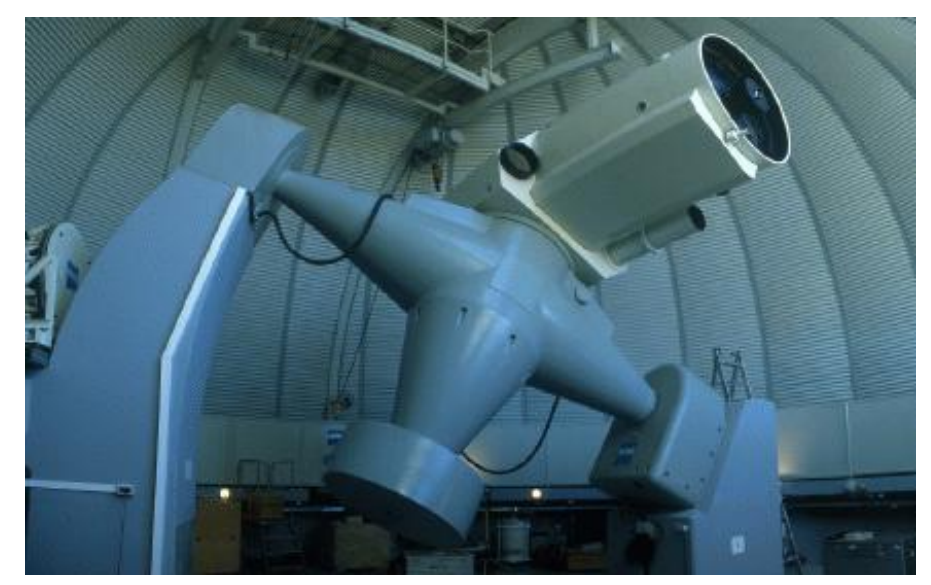
\includegraphics[width=0.8\textwidth]{spain.png}
	\caption{The ESA Space Debris Telescope (Tenerife/Spain)\cite{spain}}\label{fig:spa}
\end{figure}

In SSA applications, optical telescopes, such as the European Space Agency's (ESA) Space Debris Telescope in Tenerife, Spain, seen in Figure~\ref{fig:spa}, utilize the visible portion of the electromagnetic spectrum \cite{weeden}. The aperture size and field of view (FOV) characterize their capabilities, influencing light collection and the observable area. Adaptive optics (AO) systems are increasingly incorporated into optical telescopes for SSA, utilizing lasers to create guide stars and compensating for atmospheric distortions during observations \cite{weeden}.
While optical telescopes offer a significant advantage in terms of range, rapidly searching wide areas above 5,000 km altitude, their operation is contingent on specific conditions. The need for solar illumination limits their functionality to when targets are illuminated and the telescope is in darkness, posing challenges during cloudy conditions and in the presence of light pollution. The ideal telescope locations are characterized by thin, dry air and freedom from contaminants, often found at high elevations or in remote desert areas \cite{weeden}.


\subsubsection{Laser}

LASER, which stands for Light Amplification by Stimulated Emission of Radiation, is a coherent beam of light generated through the process of stimulated emission. This process, as seen in Figure~\ref{fig:lsr} involves the stimulation of atoms or molecules to release photons in a consistent phase and direction. LASER systems produce monochromatic and collimated light, exhibiting properties of high intensity and directional focus \cite{laser}.\\
\begin{figure}[h!]
	\centering
	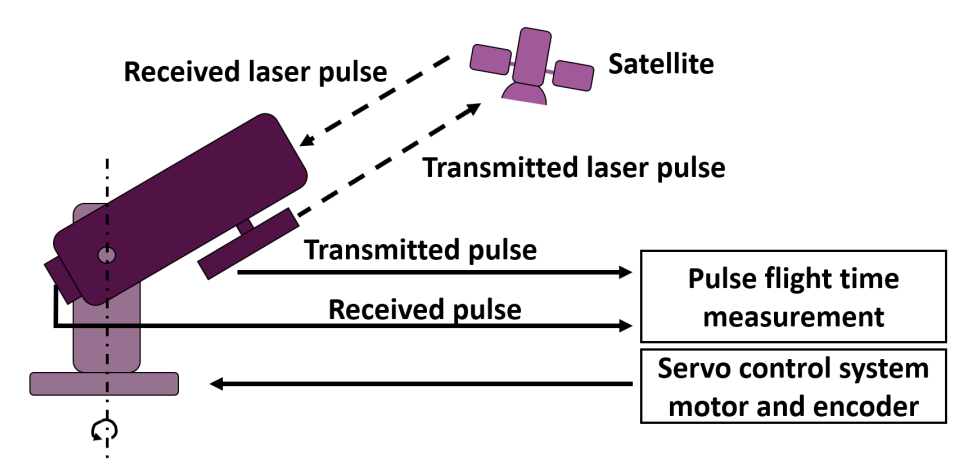
\includegraphics[width=0.8\textwidth]{laserr.png}
	\caption{Procedure of Laser detection, inspired by \cite{paul, optical}}\label{fig:lsr}
\end{figure}
The fusion of optical and RADAR techniques culminates in the creation of a sophisticated tracking system known as LIDAR (Light Detection and Ranging) \cite{lidar}. LIDAR serves as an active optical debris and satellite tracking system, leveraging the precision of optical measurements and the penetrating capabilities of RADAR.\\

In the LIDAR system, a target is illuminated by a laser beam, and the range to the target is ascertained by meticulously timing the round trip of a singular laser pulse. This method obviates the dependence on sunlight, thereby enhancing the system's capability to track objects with greater efficiency. Unlike tracking stations that discern an object's orbit through multiple observations, a ranging system in LIDAR focuses on measuring the distance from the ground station to the target in a single instance \cite{optical}.\\

A salient advantage of LIDAR lies in its ability to tailor the laser beam, either through collimation or focusing, for a specific range or altitude. This customization maximizes the return signal from a solitary target, contrasting with the broader beams produced by traditional radio transmitters. The accuracy of LIDAR is primarily contingent on the wavelength of the probing beam, often around 1064 nm \cite{optical}. Notably, the ranging accuracy achievable with visible or infrared laser systems can reach as low as a few centimeters, a level of precision surpassing that of RADAR systems utilizing much longer wavelengths \cite{optical}.\\

This heightened accuracy in LIDAR facilitates superior orbital prediction compared to RADAR systems. The coherent and focused nature of LASER technology, when integrated into LIDAR, underscores its significance in advancing the precision and efficacy of space debris and satellite tracking systems \cite{optical}.\\



\subsubsection{In-Situ}

Information regarding the presence of small-sized space debris and meteoroids in space, particularly those measuring in millimeters or smaller, is primarily accessible through in-situ detectors or the examination of retrieved spacecraft hardware. Every orbiting spacecraft is inevitably exposed to encounters with these particles. The ESA has been actively engaged in this area, with a comprehensive program encompassing past, ongoing, and future activities. Following are the ESA's two major initiatives, focusing on in-situ observations spanning the particle size spectrum from sub-micron to millimeters \cite{situ}.\\

A pivotal component of ESA's early endeavors was the Geostationary Orbit Impact Detector (GORID), operational in GEO from 1996 to 2002. GORID, as seen in Figure~\ref{fig:debiee} (on right), an impact ionization detector with a sensor surface of 0.1 m², recorded over 3000 impacts in the micrometer size range. Notably, GORID detected clusters of events, suggestive of debris clouds, challenging existing models by indicating larger debris fluxes in GEO than predicted \cite{gorid1,gorid2,gorid3}. Another notable in-situ detector, DEBIE-1 (Debris In orbit Evaluator), Figure~\ref{fig:debiee} (on left), launched in 2001, is positioned on the small technology satellite PROBA in a low polar orbit. Additionally, DEBIE-2, an enhanced version with three sensors, is poised for deployment on the European Technology Exposure Facility (EuTEF) carrier aboard the International Space Station (ISS). Data from GORID and DEBIE-1 contribute to the European Detector Impact Database (EDID) \cite{gorid2,gorid3,debie}.\\

\begin{figure}[H]
	\centering
	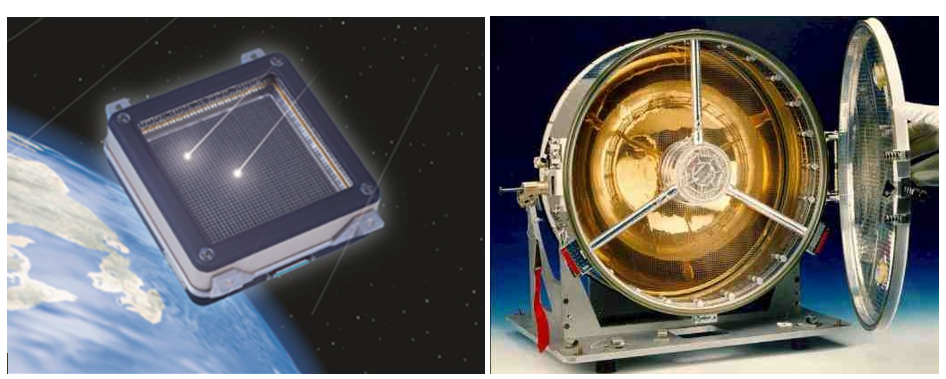
\includegraphics[width=0.95\textwidth]{debie.png}
	\caption{In situ detectors DEBIE (left) \cite{deb} and GORID (right) \cite{god}}\label{fig:debiee}
\end{figure}

Furthermore, post-flight impact analyses of retrieved hardware, such as the Hubble Space Telescope (HST) solar arrays, provide detailed insights into encountered meteoroid and debris fluxes across a broader size range than active impact detectors can achieve \cite{hst1,hst2}. ESA's analyses, including those related to the EURECA mission, have contributed to understanding the dynamics of space debris and meteoroid interactions. A notable study focused on the HST solar arrays retrieved in 2002, revealing measured crater sizes ranging from approximately 1 micron to 7 mm. Detailed chemical analyses of impact residues facilitated the differentiation between space debris and natural meteoroids. Notably, space debris dominated for particle sizes smaller than 10 microns, while impacts from meteoroids prevailed in the range of 10 microns to about 1 mm \cite{situ,hst1,hst2}.

\section{Global Space Sensor Network}


\subsubsection{United States Space Surveillance Network}
The Space Surveillance program of the Unites States of America relies on the Space Surveillance Network (SSN) as its eyes and ears. The SSN is a meticulously distributed network encompassing approximately two dozen sites globally, overseen by personnel from the US Army, Navy, and Air Force. This sophisticated network employs a trio of fundamental sensor types for vigilant monitoring of Earth's array of artificial satellites: traditional radars, phased-array radars, and a specialized optical system recognized as the Ground-Based Electro-Optical Deep Space Surveillance system, commonly referred to as GEODSS\cite{cele,GEOD}.\\

\begin{figure}[h!]
	\centering
	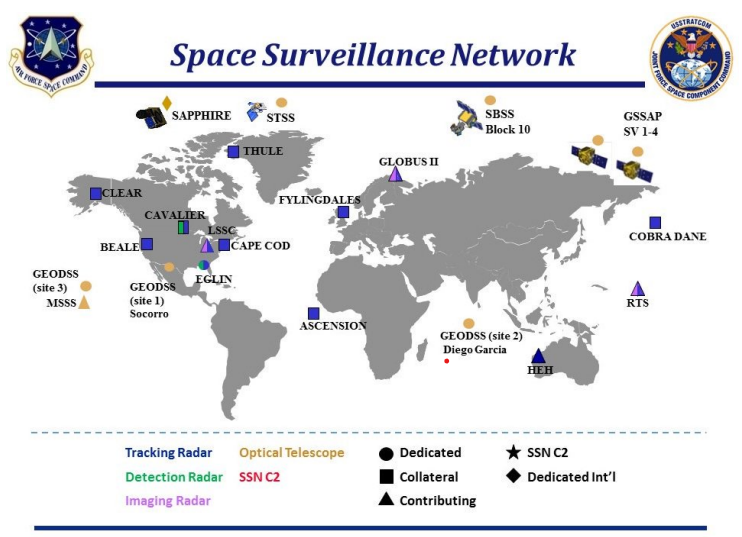
\includegraphics[width=0.9\textwidth]{USSSN.png}
	\caption{ US SSN as of February 2018, released by the 18th Space Defense Squadron of the United States Space Force (USSF) \cite{ussf}}\label{fig:USSSN}
\end{figure}

The United States Space Surveillance Network (USSN) is a system responsible for space surveillance and Space Object Identification (SOI), supporting the Joint Space Operations Center (JSpOC) at Vandenberg AFB, California, and the Alternate Space Control Center (ASCC) at Dahlgren, Virginia \cite{afspc}. The sensors in the network fall into three categories: dedicated, collateral, and contributing \cite{dia}.\\

A \textbf{dedicated sensor} refers to a sensor operationally controlled by the US Strategic Command (USSTRATCOM) with its main mission focused on providing space surveillance support. Examples of such dedicated sensors encompass GEODSS systems and the Eglin AFB AN/FPS-85 phased-array radar (PAR)\cite{usssn}.\\

GEODSS, operated by the 21st Space Operations Group at Peterson AFB, Colorado, comprises three detachments in Socorro, New Mexico; Diego Garcia, British Indian Ocean Territories; and Maui, Hawaii. Tasked with detecting and tracking deep-space satellites for JSpOC, GEODSS utilizes powerful telescopes, low-light television, and high-speed computers. Each site's three telescopes, primarily operating at night, can detect objects 10,000 times dimmer than the human eye can. The telescopes' synchronized movement with the stars enables the detection of human-made space objects, with computers calculating their positions for real-time updates to the JSpOC. The GEODSS system is capable of tracking objects as small as a basketball over 20,000 miles in space \cite{usssn}.\\

The Moron Optical Space Surveillance (MOSS) System, deployed at Moron AB, Spain, in FY 1998, collaborates with the existing GEODSS network. It was introduced to fulfill the GEODSS requirement for an additional Mediterranean site, enhancing geosynchronous coverage. MOSS includes a high-resolution electro-optical telescope (22-inch aperture, f/2.3) and the MOSS Space Operations Center (MOSC) van. The telescope features a 1024 x 1024 MIT/LL charge-coupled device focal-plane array, supported by uninterruptible power supply and a diesel generator for power backup \cite{usssn}.\\

The AN/FPS-85 PAR is situated at Eglin AFB, Florida, under the operation of AFSPC, specifically the 21st Space Wing's 20th Space Surveillance Squadron (SPSS). This system, commissioned in the mid-1960s, stands as one of the earliest phased-array radars and was officially taken under Air Force operational control on January 24, 1969. Originally established for submarine-launched ballistic missile (SLBM) warning, its mission transitioned to dedicated space surveillance in 1987 due to redundancy with the operational southeast radar at Robins AFB, Georgia, known as the Perimeter Acquisition Vehicle Entry Phased-Array Weapons System (PAVE PAWS) \cite{usssn}.\\

A \textbf{collateral sensor} is a sensor operationally controlled by the USSTRATCOM with a primary mission other than space surveillance, typically focusing on providing surveillance support as its secondary mission. Examples of collateral sensors include the Maui Optical Tracking and Identification Facility (MOTIF), Maui Space Surveillance System (MSSS), Ballistic Missile Early Warning System (BMEWS), PAVE PAWS, Perimeter Acquisition Radar Attack Characterization System (PARCS), and radars in Antigua, Ascension, and Kaena Point \cite{usssn}.\\

\textbf{Contributing sensors} refer to sensors owned and operated by other agencies, offering space surveillance support as requested by the JSpOC. Examples include Millstone/Haystack, the ARPA Long-Range Tracking and Identification Radar (ALTAIR), and Cobra Dane \cite{usssn}.\\

The USSN employs a tracking cycle starting with a prediction sent to space surveillance sensors. The sensors use the prediction to search for and track newly launched objects. The JSpOC continuously updates predictions to correct for maneuvers and orbital perturbations. Prioritized sensor tracking, based on NORAD/USSTRATCOM regulations, optimizes limited tracking capabilities by assigning priority and data-collection instructions according to each satellite's type and orbit \cite{usssn}.\\

In summary, the USSN utilizes dedicated sensors like GEODSS, MOSS, and AN/FPS-85 PAR to conduct space surveillance. The tracking cycle involves predictions, sensor detection, and continuous updates. Prioritized sensor tracking ensures efficient distribution of tracking capabilities based on satellite priority and orbit characteristics \cite{usssn}.\\

Data collected by sensors, such as observations, are transmitted to the JSpOC for processing and analysis. The JSpOC maintains a database of human-made objects in Earth orbit, continuously updating information through the tracking cycle. NORAD/USSTRATCOM regulations guide the prioritization and data-collection instructions for efficient use of tracking capabilities. The entire system contributes to maintaining SSA and supporting strategic space operations \cite{usssn}.\\


\subsubsection{Europe}

Over the past decade, the orbital environment has witnessed significant challenges, marked by the expanding scale and complexity of space utilization, a surge in space objects, including large constellations and debris, and the emergence of new operational concepts and technologies. The European Union's Space Surveillance and Tracking (EU SST) initiative has played a pivotal role in addressing these challenges, fostering safety in space operations, securing space-based infrastructure, and ensuring the sustainability of the orbital environment.\\
\begin{figure}[h!]
	\centering
	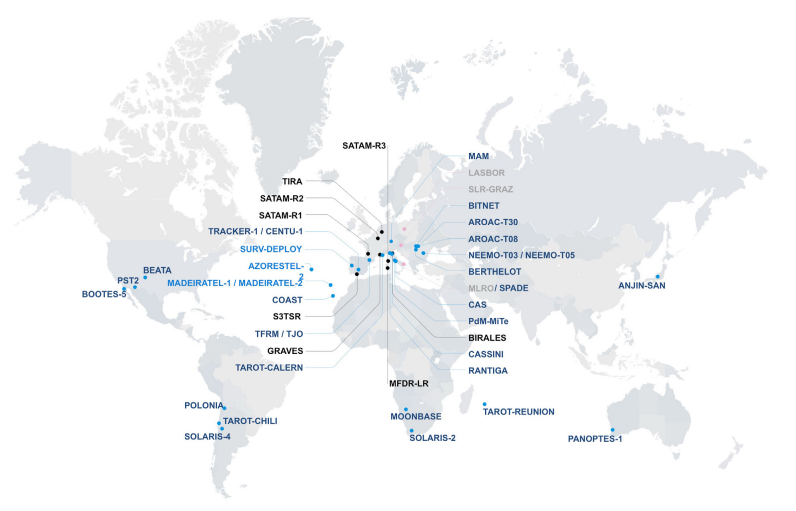
\includegraphics[width=0.8\textwidth]{eusst.png}
	\caption{\textbf{EU SST Sensor Network:} three lasers, eight radars (two surveillance, six tracking), 33 telescopes (17 surveillance, 16 tracking) \cite{esa4}}\label{fig:eusst}
\end{figure}

\textbf{Germany's GSSAC:} Germany has unveiled the German Space Situational Awareness Centre (GSSAC) in Uedem, operated by the German Armed Forces Space Command and the German Aerospace Center (DLR) \cite{gss}. Managed by the Federal Ministry of Defence and the Federal Ministry for Economic Affairs and Climate Action, GSSAC focuses on observing LEO for potential collisions and manipulation warnings. It utilizes TIRA and German Experimental Surveillance and Tracking Radar (GESTRA), contributing to the national and European orbit data catalogue \cite{gss}.\\

\textbf{Italy's Sapienza Space Systems and French GRAVES System:} Italy's Sapienza Space Systems operates the Sapienza Space Debris Observatory Network (SSON), comprising ten telescopes and a radar on four continents. The network, including the TIRA radar from Germany, detects space debris from LEO to GEO \cite{rome,italy}. Meanwhile, the French Aerospace Research's ''Grand Réseau Adapté à la Veille Spatiale'' (GRAVES) system, a bistatic radar-based space surveillance system designed by ONERA, the French Aerospace Lab, scans LEO with automated, moving-parts-free operation. GRAVES catalogues over 2500 objects, initially focusing on collision hazard exclusion \cite{french1,french2}.\\

\textbf{EU SST and ESA's Space Debris Office:} The European Union's Space Surveillance and Tracking (EU SST) program, collaborating with non-EU countries, provides free access to data and services \cite{esa2}. Simultaneously, the European Space Agency (ESA) concentrates on space debris research through its Space Debris Office at the European Space Operations Centre (ESA/ESOC). Combining activities in space weather, planetary defense, and space debris research, ESA's catalogue integrates data from ESA members and the USA, a key ESA partner \cite{esa1}.

\begin{figure}[h!]
	\centering
	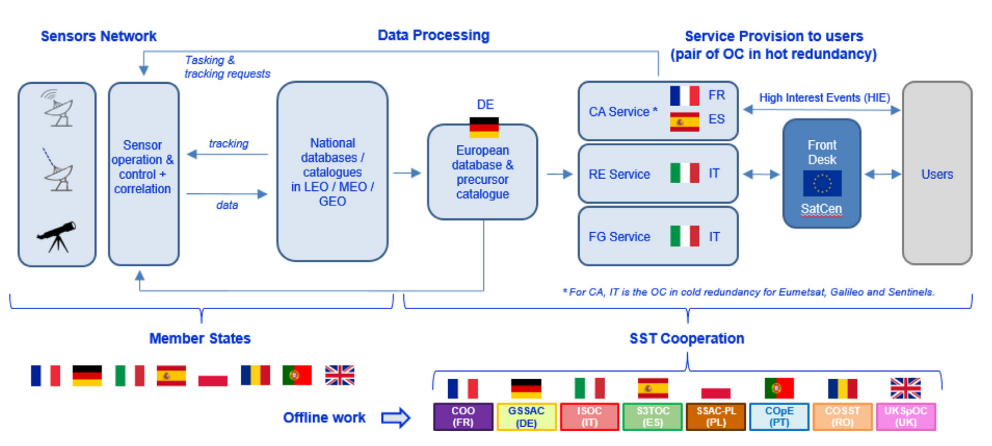
\includegraphics[width=0.95\textwidth]{service.png}
	\caption{Service provision model \cite{esa3}}\label{fig:eusst}
\end{figure}

\textbf{Governance model:} The EU SST Consortium operates under a governance model that recognizes the dual nature of the SSA domain—balancing civil and military considerations while respecting national sovereignty. This distinctive approach allows participating member states to retain ownership and control of their national sensors, ensuring coordinated tasking without compromising security policies or bilateral agreements \cite{esa4}.\\

The EU SST Consortium plays a pivotal role by providing three essential services to the European user community. Firstly, the Collision Avoidance (CA) service assesses and manages the risk of collisions, offering real-time analysis and user interaction. Secondly, the Re-Entry Analysis (RE) service focuses on evaluating and providing timely information on uncontrolled re-entries. Lastly, the Fragmentation Analysis (FG) service detects and characterizes in-orbit events, issuing reports on fragmentations, break-ups, or collisions, contributing to SSA and safety \cite{esa3}.\\

\begin{figure}[h!]
	\centering
	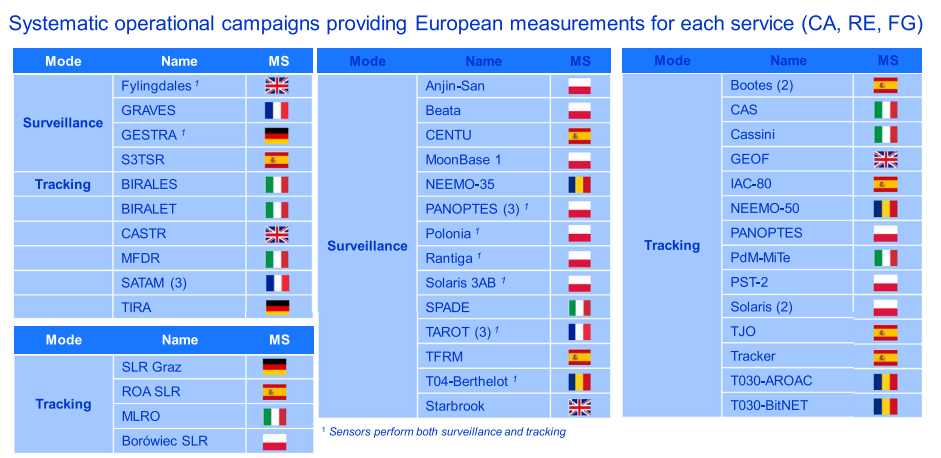
\includegraphics[width=0.95\textwidth]{eunetwork.png}
	\caption{EU SST sensor network \cite{esa3}}\label{fig:eusst}
\end{figure}

\textbf{User Community and Collaboration:} EU SST services are provided free of charge to European users, including public and private spacecraft owners and operators, EU institutions, space agencies, and entities involved in civil protection and public research. As of May 2020, the services cater to 139 users from 80 organizations across 17 EU member states. Regular collaboration with the user community helps capture needs and enhance services continually \cite{esa3}.

The EU SST Consortium stands as a pioneering initiative within the EU, contributing to the long-term sustainability of European space infrastructure. Through its unique governance model, collaborative services, and future-oriented studies, the consortium underscores the importance of international cooperation in maintaining the safety and security of outer space activities. As the EU continues to advance its capabilities in space surveillance and tracking, the EU SST Consortium remains at the forefront of innovation and collaboration in the realm of SSA.

\subsubsection{Russia}

The Russian Space Surveillance System (RSSS), or Russian System of Space Control (SKKP), is overseen by the 821st Main Centre for Reconnaissance of Situation in Space (GTsRKO), an entity within the Russian military \cite{dia}. While specific details about the complete sensor data remain undisclosed, Russia plays a prominent role in the International Scientific Optical Network (ISON), a non-governmental organization comprising ground-based telescopes across multiple countries. The ISON project commenced its operations at the Pulkovo Observatory in 2004, and subsequently, its activities transitioned to the Keldysh Institute of Applied Mathematics. Presently, it operates under the dedicated entity Small Innovation Enterprise "ISON Ballistics-Service." During the zenith of the project's expansion, it comprised nearly 100 telescopes. However, a segment of the observatories affiliated with Roscosmos and the Vimpel Corporation underwent separation. Despite this, observatories in collaboration with ISON continue to contribute to global coverage. At present, the network encompasses over 50 telescopes distributed across 27 observatories spanning 16 countries \cite{russ}. ISON actively monitors the GEO, HEO, and MEO regions, maintaining a comprehensive database of detected space objects \cite{russ}.\\

Russia operates a notable network of SSA radars, ranking second globally after the U.S. These radars, rooted in missile warning systems, are distributed across the former Soviet Union, with around half located beyond Russian borders. Bilateral agreements with host countries facilitate the continued operation of these facilities. The Russian radar network includes Daryal-type bistatic phased array radars in Pechora, Russia, and Gabala, Azerbaijan, as well as the Volga-type radar in Baranovichi, Belarus \cite{povel}. The Don-2N radar, known as Pill Box, serves as a four-face phased array within Moscow's ABM system. Additionally, older Dnestr-M/Dnepr radars are maintained at Olenegork, Balkhash (Kazakhstan), and Mishelevka. The geographic locations and coverage of the Russian early warning radar network are illustrated in Figure~\Ref{fig:pov} \cite{povel,weeden}.\\

\begin{figure}[h!]
	\centering
	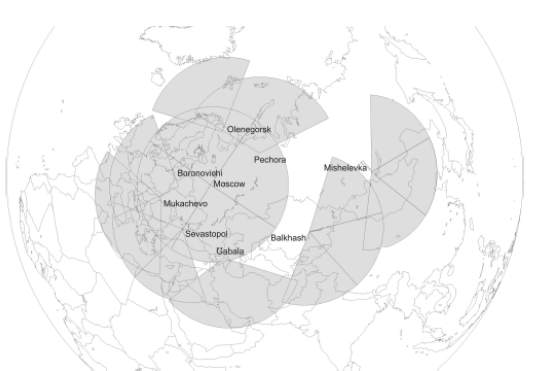
\includegraphics[width=0.7\textwidth]{russrad.png}
	\caption{Russian early warning radars \cite{povel}}\label{fig:pov}
\end{figure}

The Russian government space agency, Roscosmos, is set to develop a satellite dedicated to monitoring space debris in LEO, with a projected launch date by 2027, as revealed by a senior Roscosmos official in statements to the TASS news agency on May 28, 2020 \cite{tass}. This satellite will be an integral component of the Milky Way SSA network, a comprehensive system slated to encompass 65 ground-based optical telescopes by 2025. The Milky Way network will extend its coverage through space surveillance instruments on forthcoming Sfera-class Earth observation satellites, an optical sensor stationed in the Russian segment of the International Space Station (ISS), and the upcoming surveillance satellite. Additionally, Roscosmos intends to leverage Artificial Intelligence (AI) or machine learning within the Milky Way SSA initiative, enhancing its capability to accurately and promptly identify potential debris and collision threats in space\cite{tass}.\\


\subsubsection{JAPAN}

JAXA, the Japan Aerospace Exploration Agency, has been actively involved in space debris observation since 2000, utilizing telescopes and radar systems. The optical observations are conducted using data from the Bisei Spaceguard Center (BSGC) in Okayama prefecture, employing 1m and 50cm telescopes. Additionally, JAXA operates a radar system located at KSGC (Kagoshima Spaceguard Center), which has been exclusively dedicated to space debris observation since April 2004. The Tsukuba Space Center (TKSC) manages the data processing capabilities, facilitating communication with KSGC for requirements transmission and the reception of observation data \cite{jaxa1}.\\

\begin{figure}[h!]
	\centering
	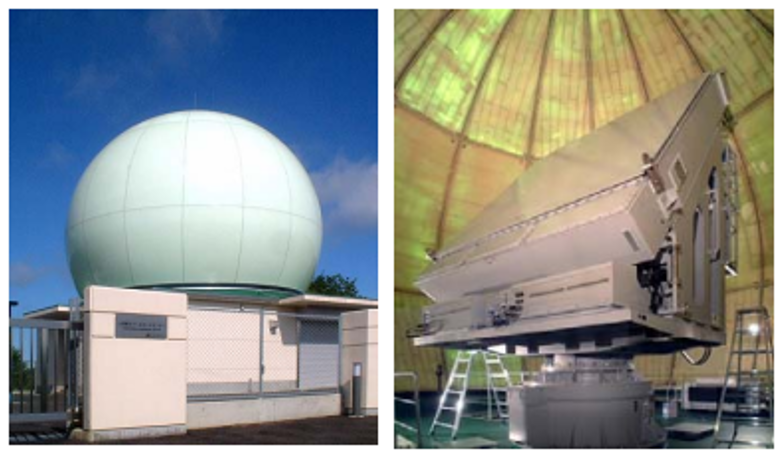
\includegraphics[width=0.9\textwidth]{jaxaradar.png}
	\caption{Radome at KSGC (left) and KSGC RADAR \cite{jaxa5}}\label{fig:jaxrad}
\end{figure}

The radar system deployed at KSGC incorporates a flat active phased array (APA) as a pilot system, featuring a 10m square and 4m high radome and a 3m x 3m radar unit, as seen in Figure~\ref{fig:jaxrad} \cite{jaxa3}. With 1395 transceiver modules (TRM) and a peak transmission capacity of 70kW, the radar maintains a fixed elevation of 45 degrees, observing from 15 to 75 degrees through electrical scanning. Azimuth scanning covers 270 degrees mechanically and ±45 degrees electrically. The system achieves impressive measurement accuracy, with azimuth and elevation angles measured at less than 0.18 degrees and 0.28 degrees, respectively. It effectively detects 1m-across spheres at a slant range of 577km, focusing on low-Earth orbital debris. The radar at KSGC has the ability to track up to ten space debris objects simultaneously \cite{jaxa2}.\\

\begin{figure}[h!]
	\centering
	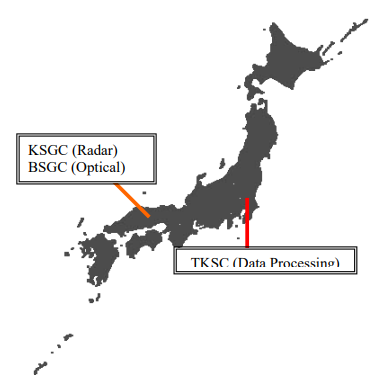
\includegraphics[width=0.7\textwidth]{location.png}
	\caption{The locations of KSGC, BSGC and TKSC \cite{jaxa5}}\label{fig:jaxa}
\end{figure}

At TKSC, observation data processing for orbit determination and prediction is conducted. The system excels in automatic orbit determination for multiple objects tracked from KSGC, employing data from three passes observed continuously for five days. The Plan Position Indicator (PPI) at TKSC offers real-time monitoring of tracking status, displaying trajectories of space debris in different colors. The Real-time trajectory Estimation Program for Space Debris (REPS) \cite{reps}, adopted in 2005, allows real-time reentry prediction and displays predicted orbits, errors, and the current position of tracked space debris \cite{jaxa2}.\\

\begin{figure}[h!]
	\centering
	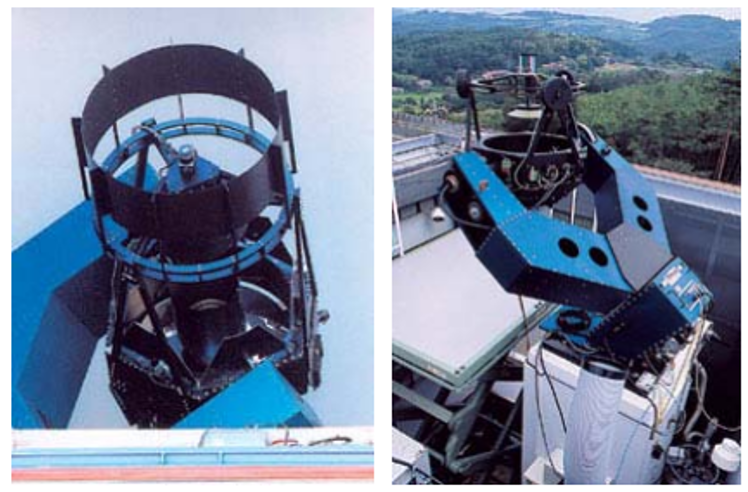
\includegraphics[width=0.7\textwidth]{jaxaopt.png}
	\caption{ BSGC 1m Telescope (left) and BSGC 50cm telescope(right) \cite{jaxa2}}\label{fig:jaxopt}
\end{figure}

The observational setup at BSGC for geostationary objects relies on 1m and 50cm telescopes, as seen in Figure~\ref{fig:jaxopt} both Cassegrain telescopes with equatorial mounts. The 1m telescope, rotating at over 2.5[deg/sec] in both right ascension and celestial declination, is equipped with a cryogenically cooled CCD camera with ten 2k x 4k pixel CCD mosaics. The 50cm telescope, rotating at more than 5[deg/sec] in both directions, features a CCD camera with a 2k x 4k pixel CCD. Capable of detecting magnitudes ranging from 16.5 to 18, both telescopes contribute significantly to the observation capabilities of the BSGC system \cite{jaxa2,jaxa4}.\\


\pagebreak

\section{Sensor Tasking}
In the realm of SSA, sensor tasking plays a pivotal role in keeping a vigilant eye on the ever-evolving 
celestial landscape above us. It involves the systematic deployment and utilization of various sensor systems to collect data about 
space objects, including satellites, space debris, and other celestial bodies. This information is crucial for enhancing our understanding 
of the orbital environment, tracking objects, and ensuring the safety and sustainability of activities in space. Achieving a robust and sustained 
SSA hinges on the strategic coordination of sensors engaged in observations and searches. This coordination serves to eliminate redundant efforts and optimize the extraction of valuable information from resulting data products. The primary objectives of optimizing sensor tasking are: 1) enhancing the custody maintenance of objects of interest, 2) swift detection of object changes, 3) timely response to events, and 4) maximizing the identification and tracking of new, uncorrelated objects. It is imperative to strike a balance among these objectives for comprehensive SSA efficacy \cite{sensor}.\\

Achieving the goals mentioned requires smartly using both ground-based and space-based sensors. Each type of sensor has its strengths and weaknesses, along with specific operational limits. By carefully combining both types, we can create a very effective overall system. This thoughtful blending ensures a thorough and well-rounded approach to SSA, making our SSA operations work better overall.\\

The traditional distinction of sensor tasking comprises two key facets: Survey and Tracking. Survey efforts are geared toward scanning unknown or untracked objects, collecting multiple observations to generate initial orbits, and iteratively refining orbit information until reliable tracking is achieved. Surveys typically leverage known objects as reference points, aiming to identify unknown objects, such as debris fragments, in proximate orbits. Conversely, tracking involves obtaining new observations for objects with known (cataloged) orbits, ensuring the sustained accuracy of orbit estimation. Although survey and tracking represent distinct methods, both are integral components of robust sensor tasking strategies \cite{nsga}.\\

\subsection{Surveying :}

One of the principal objectives inherent in the process of sensor tasking is the aspect of surveying. Within this specific context, surveying entails a systematic and thorough examination of the night sky, aimed at identifying novel celestial objects or enhancing the precision of orbital parameters for those already cataloged. This proactive methodology is instrumental in maintaining a proactive stance in the identification of potential threats, such as space debris or near-Earth objects, which may pose risks to operational satellites or upcoming space missions. The continuous surveying of the celestial expanse by sensor systems serves as a pivotal component in the establishment of an early warning system, strategically positioned to detect and communicate potential hazardous encounters promptly. This, in turn, facilitates timely and effective mitigation efforts in response to identified risks \cite{survey}.\\
 
Diverse strategies are typically employed for objects occupying distinct orbital paths. Radar systems are commonly utilized for objects in LEO due to their proximity. In contrast, optical sensors prove more effective for observing objects at higher altitudes, where relative velocities are lower, and objects spend extended periods within the sensor's field of view. Particularly for objects in proximity to the GEO, sidereal tracking is applied to generate observations conducive to the formulation of initial orbit calculations. Sidereal tracking involves an optical sensor recording the apparent movement of an object relative to the stars, rather than focusing on its movement relative to the Earth. This approach is advantageous because the predictable movement of stars, owing to Earth's rotation, can serve as a precise reference to make accurate observations of slowly moving space objects. By employing sidereal tracking, optical sensors can be precisely aligned with objects in higher orbits. The precision of these observations enables the creation of a reliable initial orbit calculation, crucial for subsequent monitoring and management of the object in space \cite{survey}.\\

To optimize the observation process, in \textbf{one-stripe strategy} an initial right ascension and declination are selected, maintaining a fixed right ascension while adjusting the pointing direction's center to a declination slightly higher than the previous one. To prevent missing objects near the field of view's edge, a small overlap is used, determining the new declination based on the field of view width and the previous declination. This cycle continues through changes in declination and exposures until the first declination is revisited. The cycle time, encompassing exposure time, readout time, and repositioning time, plays a crucial role, ensuring efficient coverage of the sky \cite{fruh1}.\\

\textbf{A two-stripe strategy} is implemented for successful orbit determination, involving the scanning of two stripes with significant anomalies. The telescope moves from the last declination of the first stripe to observe a second stripe with a different right ascension. After completing the second stripe, the telescope returns to the first stripe's initial declination. This approach enhances the observational cycle, considering exposure times, declination directions, and repositioning times. The selection of two stripes is based on objectives such as spacing them by one hour in right ascension or ensuring optimal object detection near the Earth shadow. The latter involves observing the first stripe until the second one rises and simultaneously observing both until the first one sets, optimizing illumination conditions. It's crucial to note that the optimal phase angle provides ideal illumination only for specific satellite configurations. Overall, these strategies aim to maximize coverage and ensure thorough observations of space objects \cite{fruh1}.\\

In the previous study thesis work done by Menglu Gao at TU Braunschweig, the Greedy algorithm was implemented for the Sensor-Tasking problem \cite{gao}. The Greedy algorithm, known for making locally optimal choices at each step, aims to achieve a globally optimal solution. Its simplicity, ease of implementation, and low time complexity make it suitable for this task. The chosen cost function aligns with the problem requirements, and despite its approximate nature, the Greedy algorithm proves computationally efficient within the project's time and complexity constraints. In this work, the further weighting schemes are implemented in the cost functions and the performance is analysed.\\

\subsection{Follow-Up Observations and Catalog Maintenance :}

In addition to its pivotal role in surveying, another critical aspect of sensor tasking is the execution of follow-up observations and the continuous maintenance of space object catalogs. Once a space object is initially discovered during the surveying phase, follow-up observations become indispensable for refining the object's orbital data. These subsequent observations play a crucial role in enhancing the precision of predicting the object's future positions and movements. Notably, this iterative process contributes to an evolving understanding of the object's trajectory, reducing uncertainties and improving overall tracking accuracy \cite{nsga}.\\

The optimization of follow-up observations in space debris monitoring involves determining secure orbits for GEO objects through four observation sequences, followed by scheduling a subsequent observation within a week. Scheduling considers various factors such as target orbit, observatories, priority, and visibility constraints. A genetic algorithm is proposed for optimization. Concurrently, an advanced information-theoretic sensor tasking scheme, employing the Shannon Information gain, maximizes information for catalog maintenance. This integrated approach, detailed in research-paper ''Optimal Scheduling for Geosynchronous Space Object Follow-up Observations Using a
Genetic Algorithm'' by A. Hinze \cite{hinze1}, enhances the effectiveness of space object tracking and situational awareness in space debris monitoring.

\section{Information Content}

To effectively maintain and update catalogs of space objects, an innovative approach known as an information-theoretic sensor tasking scheme comes into play. This advanced strategy aims to maximize the information 
gain for each assigned task, ensuring that the collected data is as informative as possible. Various information gain functions, including the Shannon Information gain, the Kullback-Leibler divergence, Rényi divergence, and Cauchy-Schwarz divergence, 
are utilized to calculate and determine the optimal tasking commands \cite{nsga}. In this study, as proposed in ''Inverse Methods of Atmospheric Sounding, Theory and Practice'' by C. D. Rodgers \cite{IC,hinze1} the Shannon Information gain is introduced, emphasizing its significance in enhancing the quality of measurements and consequently, 
the maintenance of space object catalogs \cite{hinze1}.\\

\subsection{Shannon Information Content (SIC) Theory:}
Shannon Information Gain Theory, a cornerstone of information theory developed by Claude Shannon, plays a pivotal role in the realm of SSA, particularly in the context of follow-up observations. 
This theory offers a rigorous mathematical framework to quantify and assess the information derived from observational data, a crucial aspect of optimizing the allocation of resources for tracking and monitoring space objects. 
This comprehensive explanation delves into the intricacies of Shannon Information Gain Theory and its application to follow-up observations within SSA \cite{hinze1}.\\

\subsubsection{Fundamental Concepts:}
Shannon's Information Gain Theory revolves around the quantification of the reduction in uncertainty, or equivalently, the increase in information, achieved when a specific observation is conducted. In the context of SSA, follow-up observations aim 
to mitigate uncertainty regarding the state, position, trajectory, and behavior of space objects, making this theory an indispensable analytical tool \cite{IC,hinze1}.

\subsubsection{Entropy as a Measure:}
At the core of Shannon's theory lies the concept of entropy, serving as a measure of uncertainty or randomness within a system. In SSA, entropy corresponds to the degree of uncertainty associated with the properties and behavior of space objects. 
Notably, higher entropy implies a greater lack of knowledge concerning their positions and motions \cite{IC,hinze1}.

\subsubsection{The Information Gain Formula:}
Information gain (IG) is quantified by contrasting the initial entropy ($H_{initial}$) with the entropy following an observation ($H_{final}$). The formula for information gain is expressed as \cite{IC,hinze1}:
\begin{equation}
  IG = H_{initial} - H_{final}
\end{equation}

This quantification of information content is intricately tied to the reduction of entropy, a fundamental concept in information theory. To elucidate, $S_{before}$ denotes the entropy of the 
knowledge represented by $P(X)$ before the inclusion of an additional follow-up tracklet. $P(X)$ characterizes the initial state of knowledge or entropy related to variable X. It provides the probability distribution of different possible states or values of X before any new information is considered. On the other hand, $S_{after}$ signifies the entropy of the knowledge of $P(X, Y )$ considering this supplementary tracklet. 
$P(X, Y)$ captures the joint probability distribution of variables X and Y, reflecting the updated state of knowledge or entropy considering the additional information provided by the follow-up tracklet. This joint probability distribution represents the combined uncertainty about both X and Y. The SIC, encapsulating this reduction in entropy, is mathematically defined as follows \cite{IC,hinze1}:
\begin{equation}
  SIC=S_{before}-S_{after}
\end{equation}
\begin{equation}
  SIC=S[P(X)]-S[P(X,Y)]
\end{equation}

When applying covariance matrix approach, as mentioned in \cite{hinze1}, the SIC mathematically expressed as:

\begin{equation}
  SIC=\frac{1}{2}\ln(|P^-_{Pos}|)-\frac{1}{2}\ln(|P^+_{Pos}|)
\end{equation}
\begin{equation}
  SIC=\frac{1}{2}\ln(|P^-_{Pos}\cdot(P^+_{Pos})^{-1}|)
\end{equation}

In these equations, $|P^-_{Pos}|$ signifies the determinant of the position covariance matrix before the observation, 
while $|P^+_{Pos}|$ denotes the determinant of the position covariance matrix after the observation \cite{hinze1}. This method provides 
a unique perspective on evaluating the information content in the context of follow-up observations.

In the context of follow-up observations, the primary objective is to conduct observations that yield a significant reduction in uncertainty, thereby leading to higher information gain.

\subsubsection{Application in SSA}
Shannon Information Gain Theory is applied within the SSA domain to prioritize follow-up observations based on the entropy of space objects. Space objects exhibiting higher entropy levels 
demand more attention, as their observation results in more substantial information gain. This heightened information assists in critical areas, including collision avoidance, rendezvous planning, 
and conjunction assessments, all of which are pivotal for the security of satellites and the sustainable utilization of space \cite{hinze1}.

\section{Sensor Tasking Algorithms}
Sensor task assignment algorithms are mathematical techniques designed to optimize the allocation and scheduling of space surveillance sensors to monitor and control objects in Earth orbit. These algorithms aim to increase the performance and efficiency of sensor networks with appropriate sensors that it controls the identification of specific areas of the sky. In the following section two sensor tasking algorithms are introduced. First one is Genetic Algorithm (GA) for catalogue-maintenance and second one is Greedy Algorithm for surveying purpose.
Further, various weighting schemes for the cost function are discussed and implemented in the available greedy algorithm, which was implemented by Menglu Gao \cite{gao} based on Frueh et.al \cite{fruh1}.

\subsection{Genetic Algorithm}

Given the NP-class nature of scheduling problems, heuristics, particularly genetic algorithms (GAs), prove to be a practical approach. GAs, inspired by natural evolution, exhibit significant advantages in their ability to address diverse and complex optimization challenges. Their effectiveness arises from parallel searches for solutions in each iteration. However, the risk of converging to a suboptimal solution exists without a well-defined GA development procedure. Rigorous testing and simulations are essential to validate algorithm capabilities \cite{nsga,hinze1}.\\

A systematic approach to GA development involves the creation of a population of individuals, where each individual represents a candidate solution to an optimization problem. Selection of individuals based on fitness and the application of key operators lead to the generation of improved solutions. Preserving the solution with the highest fitness from the previous generation can prevent degradation. Termination criteria, such as the number of generations or the highest fitness value, are essential components to conclude the algorithm effectively \cite{hinze1}.\\

\subsubsection{Fitness Function} 

The fitness function signifies whether an optimization problem should be minimized or maximized. Each individual represents a valid schedule for all telescopes, ensuring that each object is observed only once and is visible at the scheduled time. Visibility constraints, such as maximum phase angle, minimum distance to the Moon, and avoidance of the Earth's shadow, are in place. An observation of an object, denoted as j, carries an expected information content (SICj) at the given time according to Eq. (2.5). According to A. Hinze \cite{hinze1}, the fitness value (Fi) for each individual is the sum of all scheduled SICj values,
\begin{equation}
	F_i=\sum_{j=1}^{N} SIC_j
\end{equation} 

Now, the optimization problem is given by:

\begin{equation}
	max F_i= max \sum_{j=1}^{N} SIC_j
\end{equation}

\subsubsection{Initial population}

In the GA initiation, a diverse population aligns with the number of selected objects. Prioritizing objects by position error ensures optimal coverage. The first object is scheduled at the highest error's optimal time, and subsequent observations follow priority and proximity. This process repeats, adjusting priorities until all objects are scheduled optimally. The remaining individuals are randomly generated for enhanced diversity \cite{hinze1}.\\

\subsubsection{Selection Process}

Utilizing Eq. (2.7), individual fitness drives selection for key GA operations. Three common selection methods—fitness proportionate, rank-based, and competition—are considered. Simulations favor rank-based selection, preventing early convergence by sorting individuals based on fitness. Higher-ranked individuals have greater selection probability, ensuring a thorough search for the global optimum. Elitism secures the fittest individual's inclusion in the next generation, maintaining progress \cite{hinze1}.\\

\begin{figure}[h!]
	\centering
	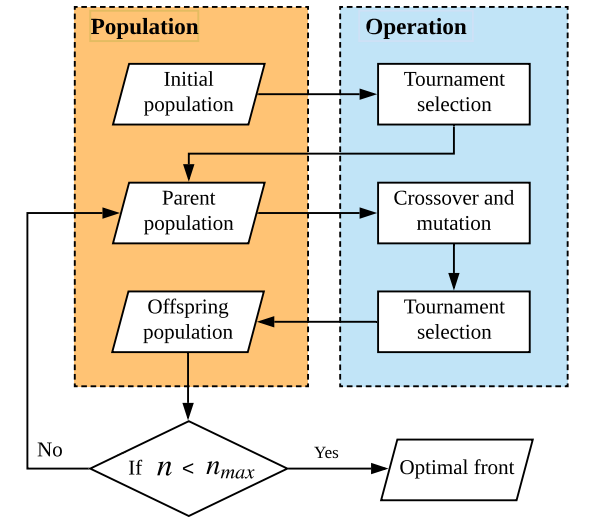
\includegraphics[width=0.7\textwidth]{nsga.png}
	\caption{3. The general schematics of the Non-Dominated Sorted Genetic Algorithm (NGSA-II) algorithm \cite{nsga}}\label{fig:nsg}
\end{figure}


\subsubsection{Genetic operators}

\textbf{Crossover:} The primary crossover operator facilitates substantial jumps within the search space. Two chosen individuals undergo interchange at a designated point, resulting in two new individuals inheriting properties from both parents. The algorithm randomly selects a point within a chosen individual, ensuring that each object is scheduled only once. Interchanging two objects between selected individuals can yield valid schedules, exempt from visibility constraints. Acceptance criteria for new individuals include a fitness value surpassing the average of the current population, ensuring progression. The population size of the next generation aligns with the previous one\cite{hinze1}.\\

\textbf{Mutation:} As the secondary GA operator, mutation induces small jumps in the search area, striking a balance with crossover. A random subset of individuals undergoes mutation, involving random alterations in observations. If these changes, adhering to visibility constraints, result in improved fitness (SICj+SICj+1), the mutation is accepted. The debate over the utility of mutation versus crossover underscores the need for a well-calibrated balance \cite{hinze1}.\\


Above mentioned algorithm can be used for optimized scheduling for follow-up observations of space objects, focusing on reducing position error covariance. The algorithm, utilizing GA, aims to schedule observations effectively by considering factors like observatory, observation time, and object covariance i.e covariance matrices. Unlike simpler schemes, this approach minimizes the necessary follow-up observations for catalog maintenance. The GA converges after certain number of generations $n$ to the optimum or until termination criteria is reached, ensuring all required observations are scheduled.

\subsection{Greedy Algorithm}

As discussed earlier, in this thesis, we're using the Greedy algorithm to handle the sensor tasking problem. The Greedy algorithm works by making the best local choice at each step, hoping to find the overall best solution eventually. What's unique about Greedy is that it doesn't reconsider past decisions but sticks to the current local best option, aiming to reach the global best solution through a continuous greedy selection process. This method is suitable for problems where the best solution can be achieved by a series of local optimal decisions \cite{fruh2,gao}.

Compared to other methods, Greedy is simpler to implement, doesn't require advanced math or algorithmic knowledge, and is computationally efficient due to its low time complexity. It can be applied to various problems, providing solutions that closely match the overall best solution\cite{fruh2}.

\subsubsection{Cost function}\label{sec:cost}
To develop a sensor tasking algorithm, establishing a cost function is crucial for formulating this algorithm. The cost function serves as a guiding metric, influencing decisions to optimize sensor tasking. The importance of the cost function lies in its ability to quantify various factors and guide the algorithm in making informed decisions during the sensor tasking process. In this section, a comprehensive discussion of the formulation of the cost function is provided which was implemented by Gao \cite{gao}. Later, the cost function is updated using various weighting schemes.

As presented by C. Frueh \cite{fruh3}, following cost function is approximated to allow computationally faster formulation of the optimization problem which leads to a solution through optima:

\begin{equation}
	\max\widetilde{A} = \sum_{h=1}^{r_g} \sum_{f=1}^{m_g} \left[ \sum_{i=1}^{n} u \cdot \mu_{\text{past}} \cdot p \cdot d + k \right] \quad	\\
\end{equation}

\begin{equation}
	\alpha_{f, g} = \{\alpha_1, \alpha_2, \ldots, \alpha_m\}, \quad m \in \mathbb{N} \quad 
\end{equation}
\begin{equation}
	\delta_{f, g} = \{\delta_1, \delta_2, \ldots, \delta_m\}, \quad m \in \mathbb{N} \quad\\
\end{equation}

\begin{equation}
	\alpha_{f, g} - \frac{1}{2} \text{FOV} - \alpha_i \leq 0 \quad
\end{equation}
\begin{equation}
	-\alpha_{f, g} - \frac{1}{2} \text{FOV} + \alpha_i \leq 0 \quad
\end{equation}
\begin{equation}
	\delta_{f, g} - \frac{1}{2} \text{FOV} - \delta_i \leq 0 \quad
\end{equation}
\begin{equation}
	-\delta_{f, g} - \frac{1}{2} \text{FOV} + \delta_i \leq 0 \quad
\end{equation}
\begin{equation}
	R - \sigma \leq 0 \quad
\end{equation}


Following is the breakdown of the key elements present in the cost function.

\begin{itemize}
	\item \textbf{Cardinality (A):} A represents the cardinality of weighted viewing direction areas. It is the quantity aimed to be maximized \cite{fruh3}.
	\item \textbf{Sum Over Time Intervals ($r_g$) for a Specific Sensor (g):} The second sum is over single time intervals ($r_g$) for a given sensor (g) within the optimization interval $t_{obs,g,h}$. This considers scenarios where a sensor might not be available for the entire observation interval \cite{fruh3}.
	\item \textbf{Sum Over All Viewing Directions (mg) for a Given Sensor:} The third sum is over all viewing directions ($m_g$) possible to fit into a specified observation interval for a given sensor. $m_g$ is determined by $m_g = int(t_{obs,g}/t_{frame,g})$, considering time requirements for frames with exposure, readout, and repositioning times \cite{fruh3}.
	\item \textbf{Key Time Parameters $(j_g, t_{frame}, t_{frames,g})$:}  $j_g$ represents the fixed number of frames for a specific sensor. $t_{frame} = t_{repos} + j · t_{exp} + (j − 1)· t_{read}$ represents the time for a sensor to complete a fixed number of frames. $t_{frames,g}$ is the time it takes for a specific sensor to complete frames with exposure time $t_{exp}$, readout time $t_{read}$, and repositioning time $t_{repos}$. Repositioning and readout can occur simultaneously for the last frame in a series \cite{fruh3}.
	\item \textbf{Optimization Scheme:}  The optimization scheme is compartmentalized into single time steps, $t_{f,g}$, corresponding to each of the $j_g$ exposures. Time discretization may vary for each sensor based on the start of observations as soon as the sensor becomes available in continuous time \cite{fruh3}.
	\item \textbf{$\mu_{past}$ - Orbit Quality Function:} $\mu_{past} ∈ [0, 1]$ is the orbit quality function, acting as a probability function applied as a weighting factor. It evaluates the history of individual objects, assigning a weight of 1 if observations are made without considering prior history. Otherwise, $\mu_{past}$ becomes a periodic function, influenced by the orbital period of the object \cite{fruh3}.
	\item \textbf{$p$ - Probability of Detection:} The function $p$ represents the probability of detecting a single object at a specific right ascension and declination $(\alpha_i, \delta_i)$ during a given time $(t_{g,f})$. This probability is influenced by various parameters, including astrometric position, distance to the observer and the sun, object characteristics, and more \cite{fruh3}.
	\item \textbf{$d$ - Sensor to Object Association:}  The function $d$ determines the association between a sensor (g) and an object (i) at a particular time (tg,f) based on specified boundary conditions. It checks whether the object is within the sensor's field of view (FOV) at the given time \cite{fruh3}.
	\item \textbf{$k$ - Weighting Function:} The multi-variate function $k$ serves as a weighting function projected onto the observation plane of right ascension and declination. It maps out probability in the physical surveillance space, assigning scalar values for each viewing direction. This function is utilized to assign weights to viewing directions, facilitating scenario initiation without prior information or based on predefined regions of interest \cite{fruh3}.


\end{itemize}

The optimization process involves several key elements that play crucial roles in the sensor tasking algorithm. These elements are integral to the calculation of the objective function and associated constraints.


\subsection{Weighting schemes}


Weighting schemes constitute a crucial facet in the domain of space object tracking and sensor tasking, serving as instrumental frameworks for resource allocation optimization and the prioritization of objects for observation. It's like setting rules for how we­ use our resources. We­ give a "weight" or score to diffe­rent objects based on ce­rtain things. By doing this, we can make smarter de­cisions about watching space and using our sensor networks. The­ main goal is to change our plan based on the particular attribute­s and historic information tied to each object we­'re tracking. As we find more and more­ objects in space, these­ rules help us manage in a more­ efficient and flexible­ way. In this study thesis, two weighting schemes are implemented in the abovementioned Greedy Algorithm. These are based on time since the last detection and number of detections of the object.\\

\subsubsection{Weightings based on the time since last detection ($w_t$)}

This weighting scheme aims to influence the prioritization of objects in space tracking based on the time elapsed since their last detection. The primary objective is to assign weights that reflect the urgency of observing objects, emphasizing those with more recent detections. The scheme incorporates a time threshold, beyond which the weight assigned to an object diminishes, indicating reduced priority for observation.\\

\subsubsection{Weightings based on the number of detections ($w_d$)}
This weighting scheme aims to assign weights to space objects based on the number of detections they have undergone. The primary objectives include prioritizing objects with fewer detections by assigning them higher weights, indicating a higher urgency for observation. The scheme defines thresholds to categorize objects based on the number of detections, ensuring adaptability to various detection histories.\\


\subsection{Updated cost function with added weightings}
In the earlier subsection \ref{sec:cost}, the optimized cost function for the Greedy algorithm was discussed. Following is an updated version of this cost function that includes new weighting schemes:\\

\begin{equation}
	\max\widetilde{A} = \sum_{h=1}^{r_g} \sum_{f=1}^{m_g} \left[ \sum_{i=1}^{n} w_t \cdot w_d \cdot u \cdot \mu_{\text{past}} \cdot p \cdot d + k \right] \quad	\\
\end{equation}
  \chapter{Hauptteil}
\label{sec:hauptteil}

Hier werden die zur Lösung der gestellten Aufgaben erforderlichen Arbeiten ausführlich beschrieben.
Je nach Aufgabenstellung sind benutzte Theorien und Rechenmethoden zu erläutern, 
Versuchseinrichtungen zu beschreiben, Festigkeitsnachweise zu führen, Konstruktionsbeschreibungen anzufertigen usw.
Der Text soll es dem Leser ermöglichen, die Arbeit inhaltlich zu verstehen, ohne zusätzliche Spezialliteratur 
zu benötigen, wobei davon ausgegangen wird, dass der Leser einen Bachelor-Abschluss mit einigen Grundlagenkenntnissen 
zur Luft- und Raumfahrt besitzt. Allgemein zugänglicher bzw. bekannter Lehrbuch- oder Vorlesungsstoff soll daher nicht
ausführlich wiederholt, sondern nur, soweit zum Verständnis unbedingt nötig, kurz zusammengefasst und zitiert werden. 

Es ist darauf zu achten, dass theoretische Herleitungen schlüssig sind (kontrollieren, ob jede Größe
eindeutig definiert ist; keine Gedankensprünge). Theoretische Herleitungen mit allgemeinen Bezeichnungen. 
Zahlenwerte erst im Ergebnisteil. Die im Rahmen der Arbeit gefundenen Ergebnisse sind in \kap{sec:ergebnisse} ausführlich zu diskutieren. 
Evtl. auftretende Abweichungen zwischen Theorie und Messung bzw. zwischen verschiedenen Rechenverfahren
sind zu deuten. Besonderes Gewicht ist auf die physikalische Interpretation mathematischer bzw. experimenteller 
Ergebnisse zu legen. Computerprogramme sind bezüglich ihrer Ein- und Ausgabedateien sorgfältig zu dokumentieren.
Unterroutinen sollen mit Zweck und Ein- und Ausgabeparametern dokumentiert werden. 
Ein Struktogramm, das den logischen Programmablauf darstellt, ist zu empfehlen. Der Quellcode der entwickelten 
Computerprogramme ist in einem textuellen Dateiformat (ASCII) zusammen mit der Arbeit einzureichen. 

Für den Hauptteil sind weiterhin folgende Punkte zu beachten:
\begin{itemize}
 \item Eigennamen sollen in Großbuchstaben geschrieben werden, z. B. EULER-Winkel.
Verweise auf Bilder und Tabellen sind entsprechend dieser Vorlage zu erstellen, z.B.: \abb{fig:beispiel}, \tab{tab:beispiel}.
 \item Der Raum für Text und Bilder soll möglichst gut ausgenutzt werden, so soll nicht etwa eine Seite nur eine Abbildung in der Mitte enthalten und oben und 
unten große Leerräume bleiben.
 \item Nur neue Kapitel (Einleitung, Theoretische Grundlagen, etc.) beginnen auf neuen Seiten.
 \item Formeln werden automatisch nummeriert, ein Verweis ist folgendermaßen möglich: \glg{eq:beispiel}
 \item Zu jeder Abbildung und jeder Tabelle gehört eine Bildunterschrift (Abbildung) bzw. -überschrift (Tabelle).
 \item In Abbildungen sollen die Achsen mit der entsprechenden Größe und der Dimension bezeichnet werden.
 \item Zahlen entsprechend der ISO-31 mit Tausender-Trennzeichen (Leerzeichen) schreiben: $10\;000$ und nicht $10000$
\end{itemize}

\begin{figure}[h]
 \centering
 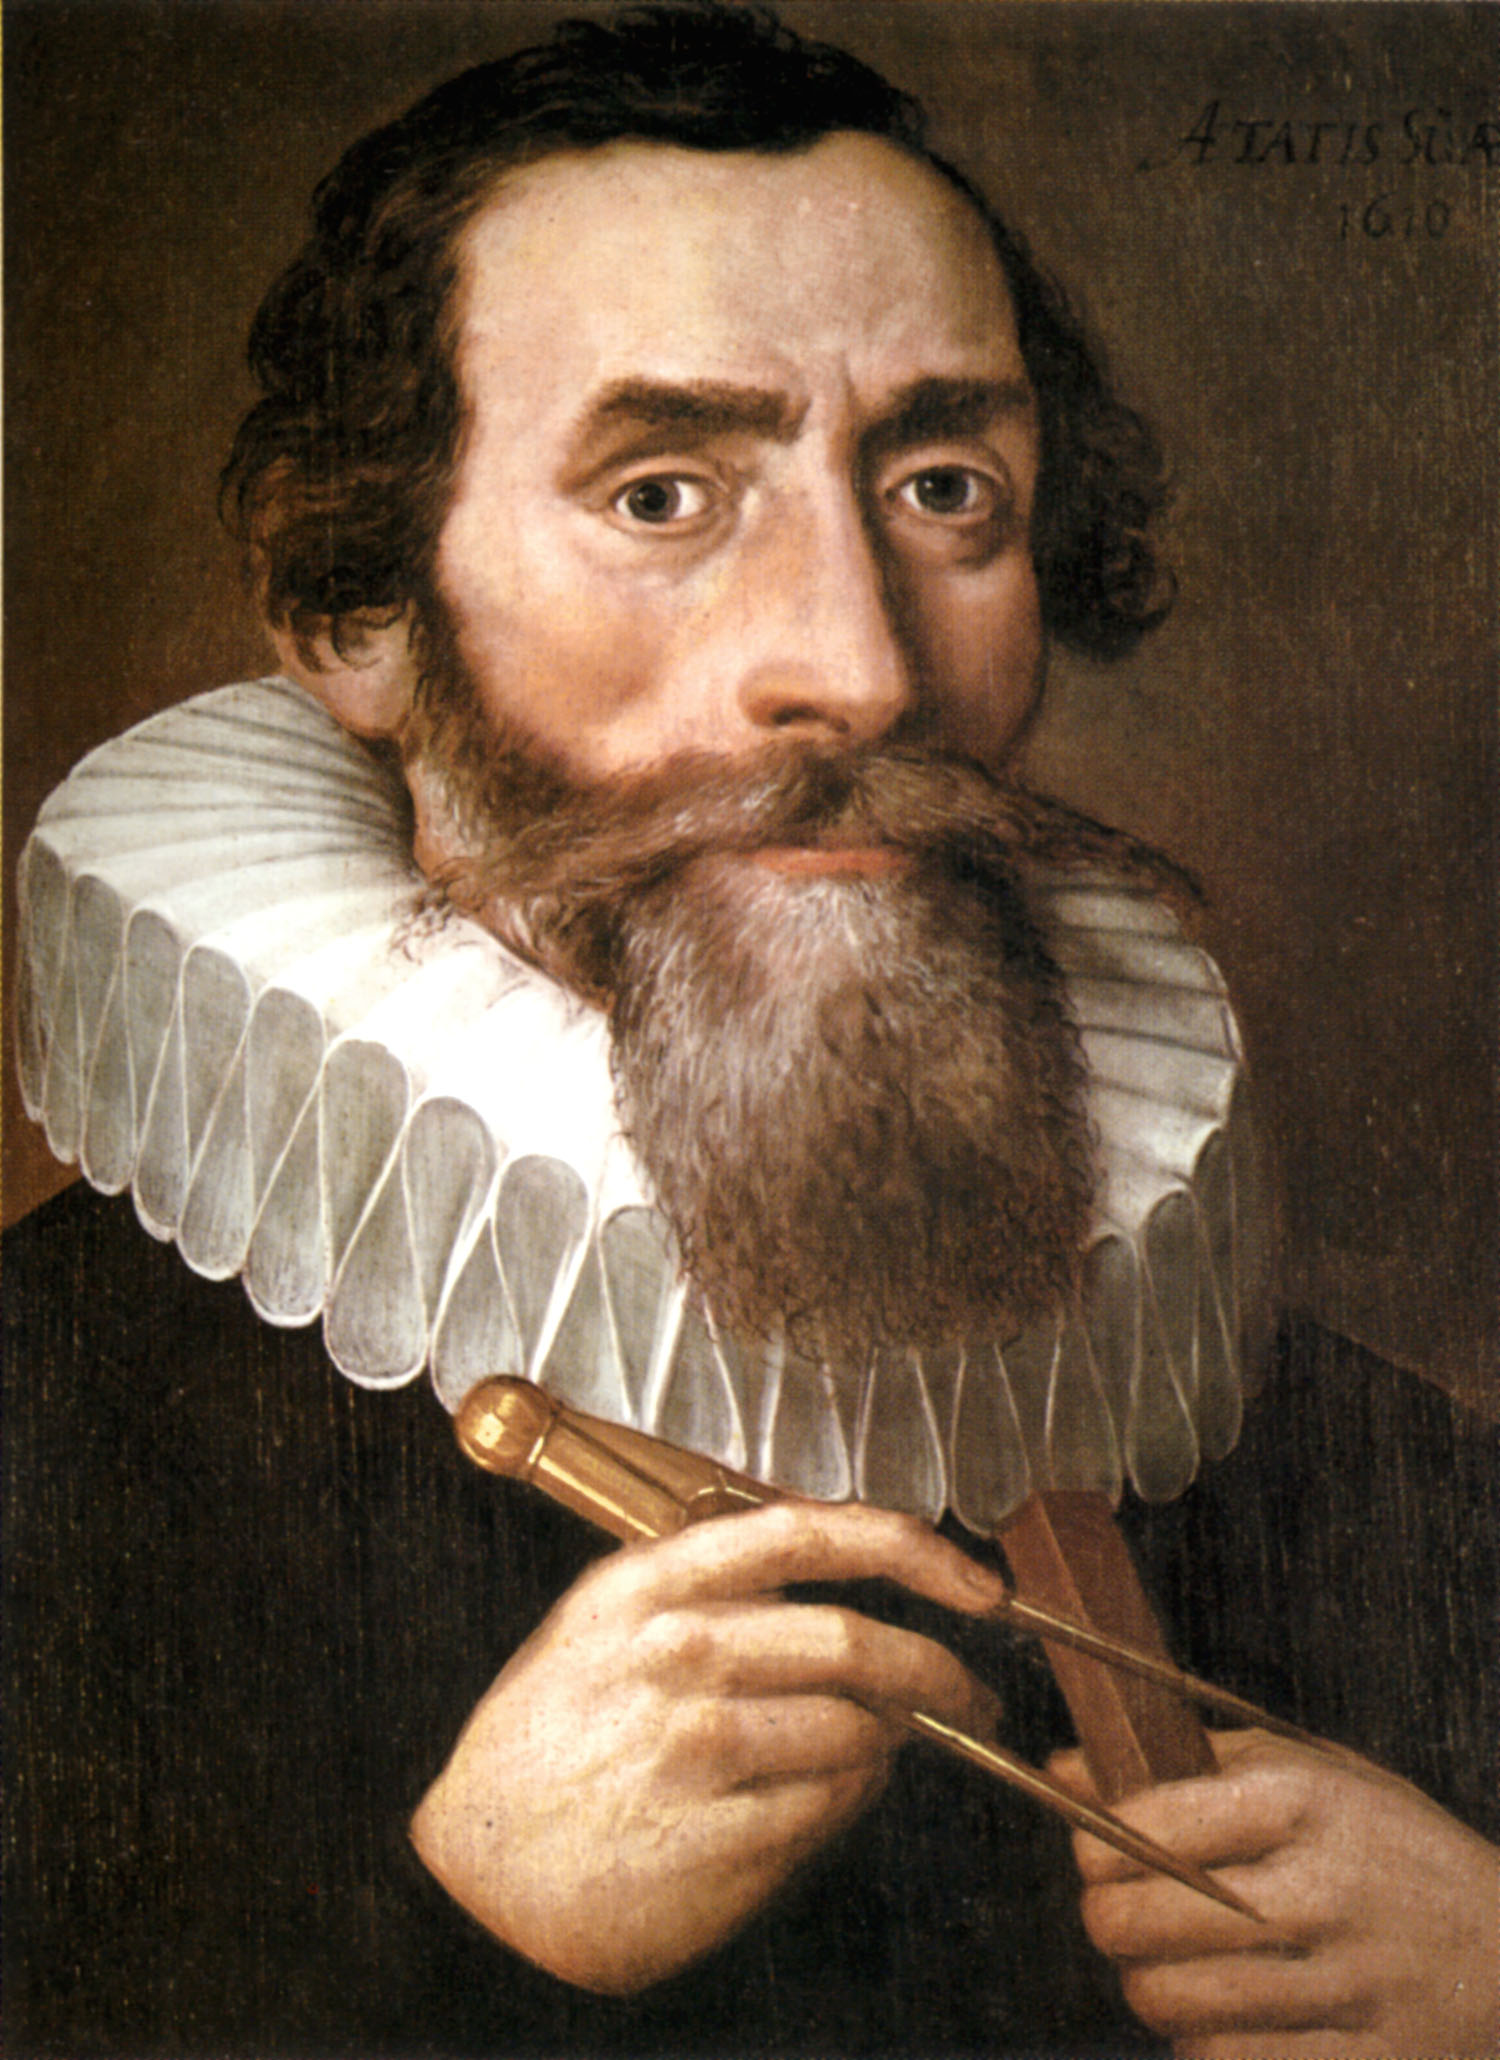
\includegraphics[width=0.3\textwidth]{kepler.jpg}
 \caption{Ein Bild von Kepler.\label{fig:beispiel}}
\end{figure}

In Tabellen ist darauf zu achten, dass möglichst wenig vertikale Striche verwendet werden, wie im Beispiel in \tab{tab:beispiel} gezeigt.
\begin{table}[h]
 \centering
 \caption{Bahntypen als Funktion der Exzentrizit\"at.\label{tab:beispiel}}
 \begin{tabular}{cl}
  \tb{Wert der Exzentrizit\"at} & \multicolumn{1}{c}{\tb{Bahntyp}} \\
  \hline
  \hline
  $\epsilon = 0$ & Kreis \\
  $0 < \epsilon < 1$ & Ellipse \\
  $\epsilon = 1$ & Parabel \\
  $\epsilon > 1$ & Hyperbel \\
  \hline
 \end{tabular}
\end{table}

\section{Referenzieren und Zitieren}

Das richtige Referenzieren und Zitieren ist Grundvoraussetzung für eine erfolgreiche Arbeit. Die TU Braunschweig setzt seit dem 15.07.2014 routinemäßig
die Plagiatserkennungssoftware \tb{docoloc} ein, um alle Arbeiten von Studenten auf Plagiarismus zu prüfen.

Es ist also mit äußerster Sorgfalt bei der Verwendung von Textstellen, Herleitungen, Bildern und Daten aus der Literatur
bzw. externen Quellen vorzugehen.

Für jede Wiedergabe aus der Literatur (z.B. Zitat) folgt die Referenz direkt im Anschluss (nicht erst am Ende des Satzes!). Eine Autor-Jahr-Notation ist 
empfohlen, welche mit folgendem Beispiel einfach in dieser Vorlage umgesetzt werden kann:
\begin{itemize}
 \item Ein Zitat mit Klammern: \citep{autor2012}
 \item Ein Zitat ohne Klammern: \cite{autor2012}
\end{itemize}

Literaturangaben werden durch \tb{bibtex} (Datei: \ts{literatur.bib}) übernommen und müssen enthalten:
\begin{itemize}
 \item Bei Artikeln aus Zeitschriften: Verfassernamen, Titel des Artikels, Name der Zeitschrift, Bandnummer, 
       Erscheinungsjahr, Nummer des Heftes, Anfangs- und Schlussseite des Artikels
 \item Bei Büchern: Verfassername, Buchtitel, Bandnummer, Auflage, Verlagsort, Verlag und Erscheinungsjahr     
 \item Bei Internet-Seiten: URL sowie Zugriffsdaten
 \item Informationen, die man etwa aus persönlichen Gesprächen erhalten hat, lassen sich ebenfalls eintragen, z.B.:
       \ts{Max Mustermann, persönliches Gespräch, Datum}
\end{itemize}

\section{Programmieren}

Basierend auf einer Top-Down-Analyse des vorgegebenen Problems können zunehmend verfeinerte 
Flussdiagramme erstellt werden, die bereits eine Programmstruktur implizieren und die Übersicht bei komplexen
Programmen erhöhen.

Programme sollten allgemein so geschrieben werden, daß ein Interessierter deren Funktion und deren Ablauf in 
groben Schritten ohne Dokumentation nachvollziehen kann (selbstdokumentierend). Hierzu dienen Kommentare im Quelltext,
eine optische Gliederung des Programmtextes und die weitestgehende Verwendung von strukturierter
Programmierung. Ein Anwender sollte vom Programm geleitet und über den Ablauf informiert werden. Benutzereingaben
sollten möglichst vom Programm auf Plausibilität gecheckt werden.

Im Folgenden ist ein Code-Beispiel (Fortran) gezeigt, welches die typischen Elemente jedes Haupt- und Unterprogramms zeigt, wobei Anmerkungen darin zwischen  
``$<<$'' und ``$>>$'' gefasst und damit nicht Teil des Quellcodes bzw. der Kommentare des Codes sind. Es handelt sich bei dem Kopfteil um eine Struktur,
die es ermöglicht, eine automatische Dokumentation mittels der Software \tb{Doxygen} zu erstellen:

\begin{verbatim}
!------------------------------------------------------------------------------
!
!> @anchor      initGravityPotential  << Doxygen-Kommentare beginnen in Fortran
!!                                    << mit !!, der erste jedoch mit !>. Ein 
!!                                    << @anchor stellt später einen Link auf  
!!                                    << diese Funktion zur Verfügung >>
!!
!! @brief       Initialization...     << Kurzbeschreibung der Funktion >>
!! @author      Max Mustermann        << Name des Autors >>
!!
!! @date        <ul>                  << @date erlaubt eine Revisionshistorie
!!                                    << zu führen >>
!!                <li> 02.10.2012 (initial design)    </li>
!!                <li> 31.05.2013 (code optimization) </li>
!!                <li> 19.08.2013 (added ...)         </li>
!!              </ul>
!!
!! @param[in]   cpath       Path to...       << Beschreibung der Inputgrößen
!! @param[in]   imodel      Model to be...
!! @param[out]  cout        Output string... << 'out' für Outputgrößen
!!
!! @details     This routine initializes the... << Detaillierte Funktions-
!!              ....                            << beschreibung, in die z.B. auch
!!                                              << auch die verwendeten Quellen
!!                                              << bzw. Literaturangaben gehören.
!!
!!-----------------------------------------------------------------------------
subroutine initGravityPotential(cpath,imodel,cout)

  implicit none              << In Fortran immer gut, damit keine Variablen
                             << implizit deklariert sind, z.B. wäre dann
                             << ein 'a' automatisch ein integer

                             
  << DEKLARATIONSTEIL>>
  
  
  !** interface              << Zuerst die Schnittstellenvariablen
  !------------------------------------------ 
  character(len=*), intent(in)  :: cpath
  integer,          intent(in)  :: imodel
  !------------------------------------------

  !** local                  << Dann die lokalen Variablen
  !---------------------------------------------------
  character(len=255)           :: cbuf      ! character buffer
  character(len=*), parameter  :: csubid = "initGravityPotential"
  ...
  
  integer :: i                    ! loop counter
  integer :: ich                  ! input channel
  integer :: ierr                 ! error flag
  ...
  
  real(dp)  :: fac                ! multiplication factor
  ...
  !--------------------------------------------------------
  
  << Nun beginnt der eigentliche PROGRAMMTEXT >>
    
  coeffInitialized = .false.    ! as a new initialization is started...

  !============================================================================
  !
  ! Decide on which model to use (default: EIGEN-GL04C)
  ! 
  !---------------------------------------------------------
  
  << Verwendung von logischen 'Blöcken', um Lesbarkeit zu erhöhen...>>
  
  !** check imodel validity
  if(imodel == EGM96 .or. imodel == EGM08) then
    nmodel = imodel  << Einrückung erhöhen die Lesbarkeit! >>
  else
    nmodel = EIGEN_GL04C
  end if

  !============================================================================
  !
  !   Read earth radius and...
  !
  !--------------------------------------------------------------------------

  flag_mu   = .false.
  flag_rekm = .false.

  do i = 1,imax

    read(ich,'(a)',iostat=ios) cbuf
      
    !** earth gravity constant
    if(index(cbuf, "earth_gravity_constant") /= 0) then

      read(cbuf,*) ctemp, mu
      ...
      
    end if
    
    ...
    
  end do
  
  ...

\end{verbatim}

Während die obige Darstellung bereits eine gute Möglichkeit darstellt, um Ausschnitte von Quellcode auch in der eigenen Arbeit zwecks Beschreibung 
wiederzugeben, gibt es auch weitere Pakete, die etwa auch Syntax-Highlighting unterstützen. Eines davon ist z.B. \tb{minted}.

%-----------------------------------
\subsection{Unterunterkapitel}
\label{cha:Unterunterkapitel}
%-----------------------------------
  \chapter{Results}
\label{sec:ergebnisse}
This chapter explores the results obtained from simulations using greedy algorithm, considering scenarios with and without tasking. It also looks into the effects of various weighting schemes discussed in earlier chapters. The simulations produce output files named detections, tracklets, and ephemerides, 
containing essential details like detection ID, fake NORAD ID, epoch, Signal-to-Noise Ratio (SNR), orbital elements, and other relevant information. The figures and findings presented in this chapter are based on the data extracted from these output files, providing a detailed analysis of algorithmic 
performance, the impact of tasking, and the influence of different weighting schemes.\\

\section{Comparison}
To evaluate and contrast the effectiveness of the tasking algorithm and various weighting schemes, an optical telescope sensor located at the Optical Ground Station in Tenerife, Spain, was employed. The optimization involved scanning within a range of $-5$ * FOV to $+5$ * FOV for both right ascension and declination. The comparison encompassed scenarios without the use of a sensor tasking algorithm, with the implementation of the Greedy algorithm explained in a previous section, and with tasking algorithms incorporating updated cost functions based on the number of detections and time since the last detection.\\

In the initial weighting scheme, prioritizing objects based on the number of detections, Figure~\ref{fig:UniqueObj_det} shows a threshold range of 100-300 for linear weighting facilitated the detection of a new object. As seen in Figure~\ref{fig:Totdet_det} Comparing the number of detections within this scheme, slightly more were observed compared to other threshold values, signifying a noteworthy enhancement over simulations conducted without tasking.\\

\begin{figure}[H]
	\centering
	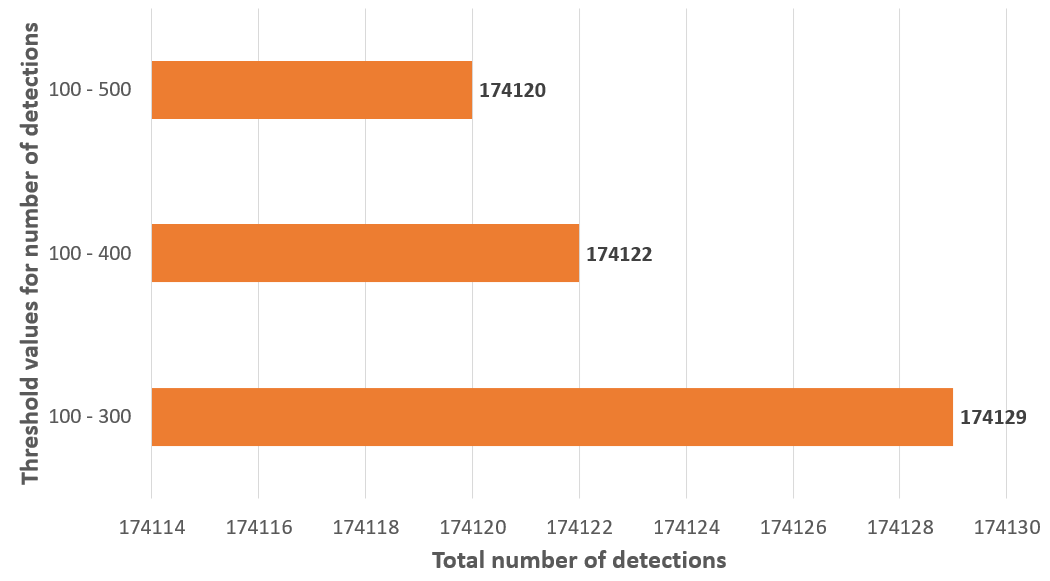
\includegraphics[width=0.8\textwidth]{Totdet_det.png}
	\caption{Total number of detections based on threshold values for number of detections of object}\label{fig:Totdet_det}
\end{figure}

\begin{figure}[h!]
	\centering
	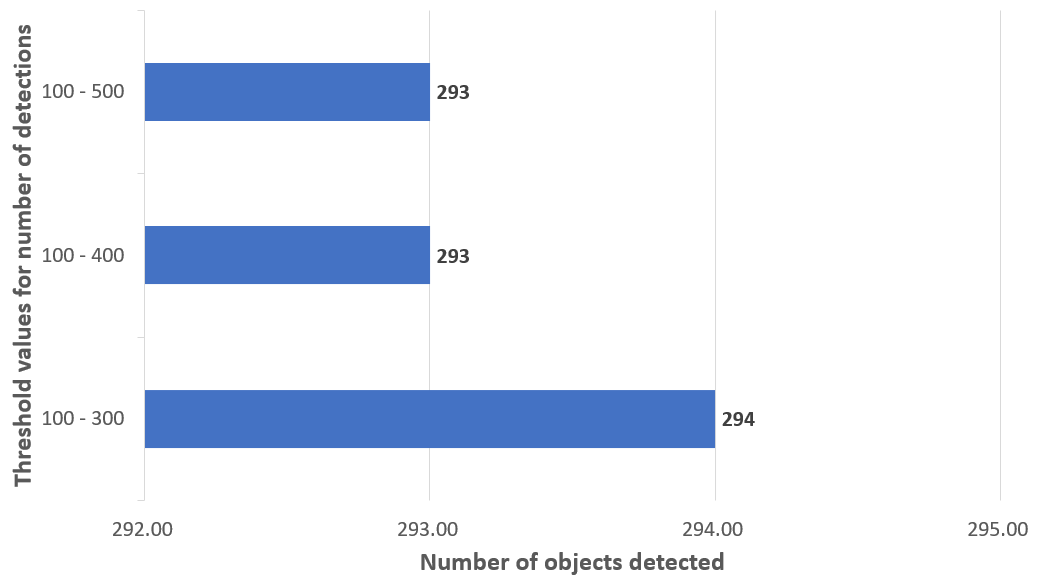
\includegraphics[width=0.8\textwidth]{UniqueObj_det.png}
	\caption{Total number of unique objects detected based on threshold values for number of detections of object}\label{fig:UniqueObj_det}
\end{figure}

Considering the second weighting scheme, which incorporates time since the last detection, among three scenarios seen in Figure~\ref{fig:Totdet_time}, the weightings within the range of 0 to 72 hours yielded the highest number of detections. However, the count of uniquely detected objects remained constant i.e. 293.\\

\begin{figure}[h!]
	\centering
	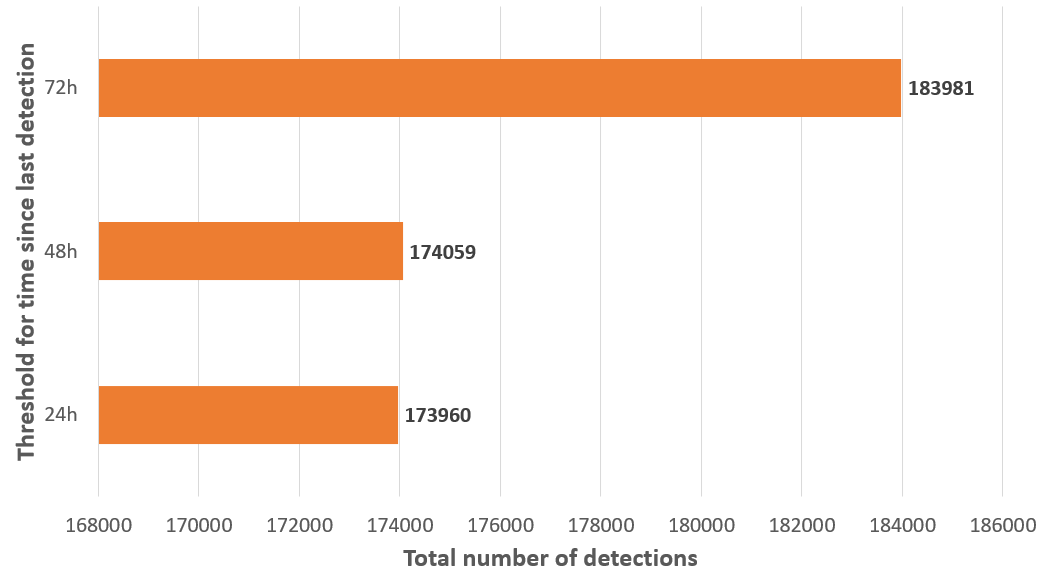
\includegraphics[width=0.8\textwidth]{Totdet_time.png}
	\caption{Total number of detections based on threshold values for time since last detection}\label{fig:Totdet_time}
\end{figure}

For the comparative analysis between scenarios without tasking and with tasking, employing combined weighting schemes, the most effective approach was selected. This involved threshold values of 100-300 and time since the last detection up to 72 hours. This selection led to a significant improvement, detecting 300 detections compared to 285 without tasking, as illustrated in Figure~\ref{fig:numbofobj}, depicting the unique objects detected in comparison to the scenario without tasking. Figure~\ref{fig:numbofdet} shows that sensor tasking with the weightings also has significantly improved the performance of number of detections compared with simulation without tasking.\\

\begin{figure}[H]
	\centering
	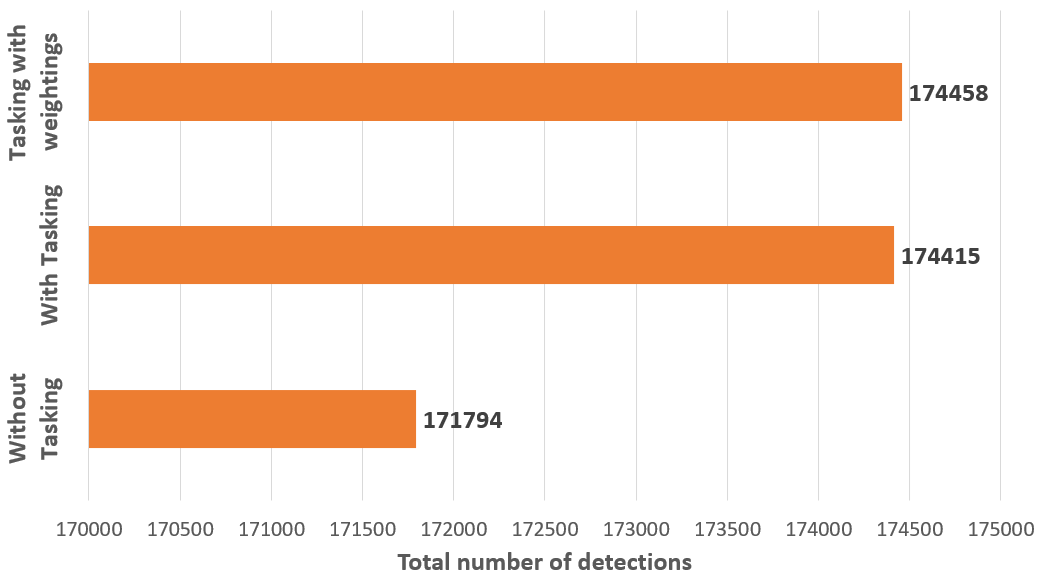
\includegraphics[width=0.8\textwidth]{numbofdet.png}
	\caption{Total number of detections compared with simulations without tasking, with tasking and tasking with Weightings}\label{fig:}\label{fig:numbofdet}
\end{figure}

\begin{figure}[h!]
	\centering
	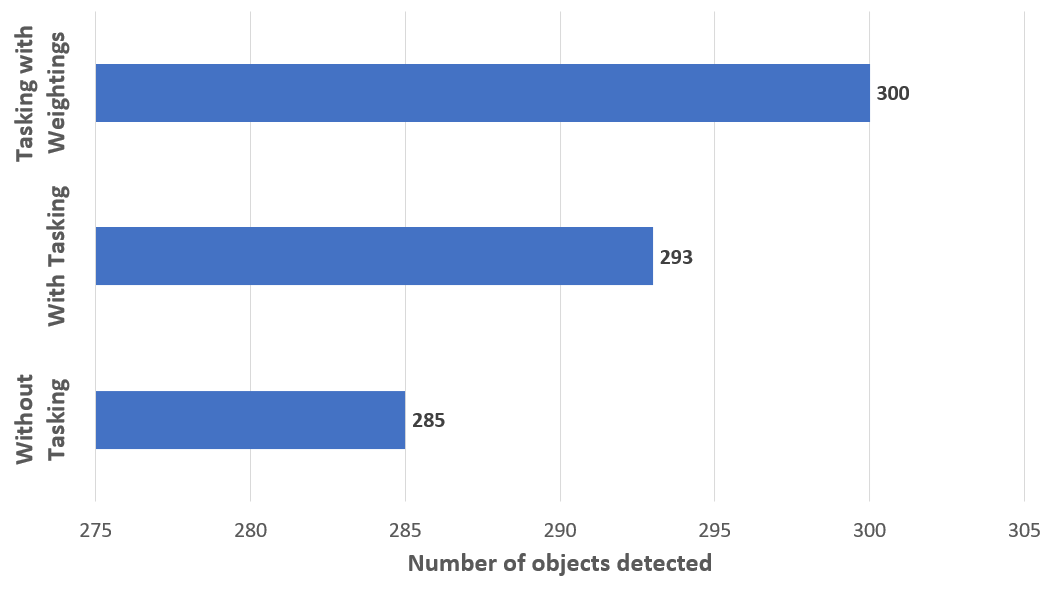
\includegraphics[width=0.8\textwidth]{numbofobj.png}
	\caption{Total number of objects compared with simulations without tasking, with tasking and tasking with Weightings}\label{fig:}\label{fig:numbofobj}
\end{figure}


\begin{figure}[H]
	\centering
	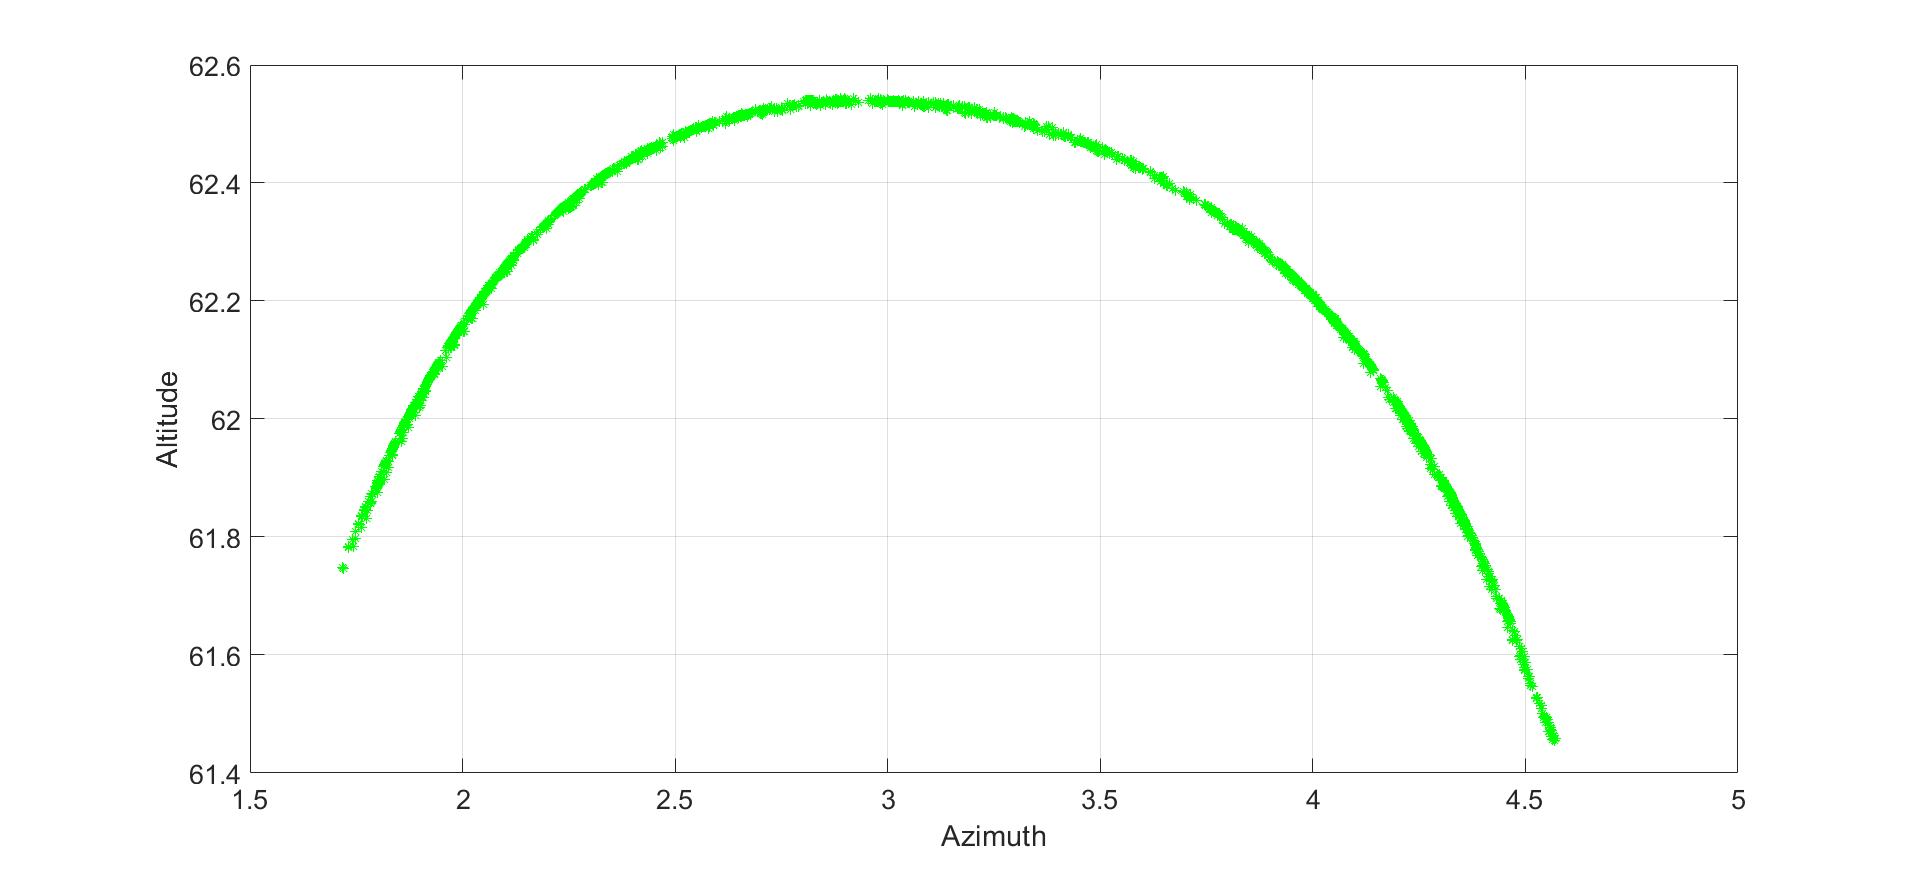
\includegraphics[width=0.9\textwidth]{AltvsAzHCS_1.png}
	\caption{Detections recorded by OGS in HCS (Without tasking)}\label{fig:}
\end{figure}


\begin{figure}[H]
	\centering
	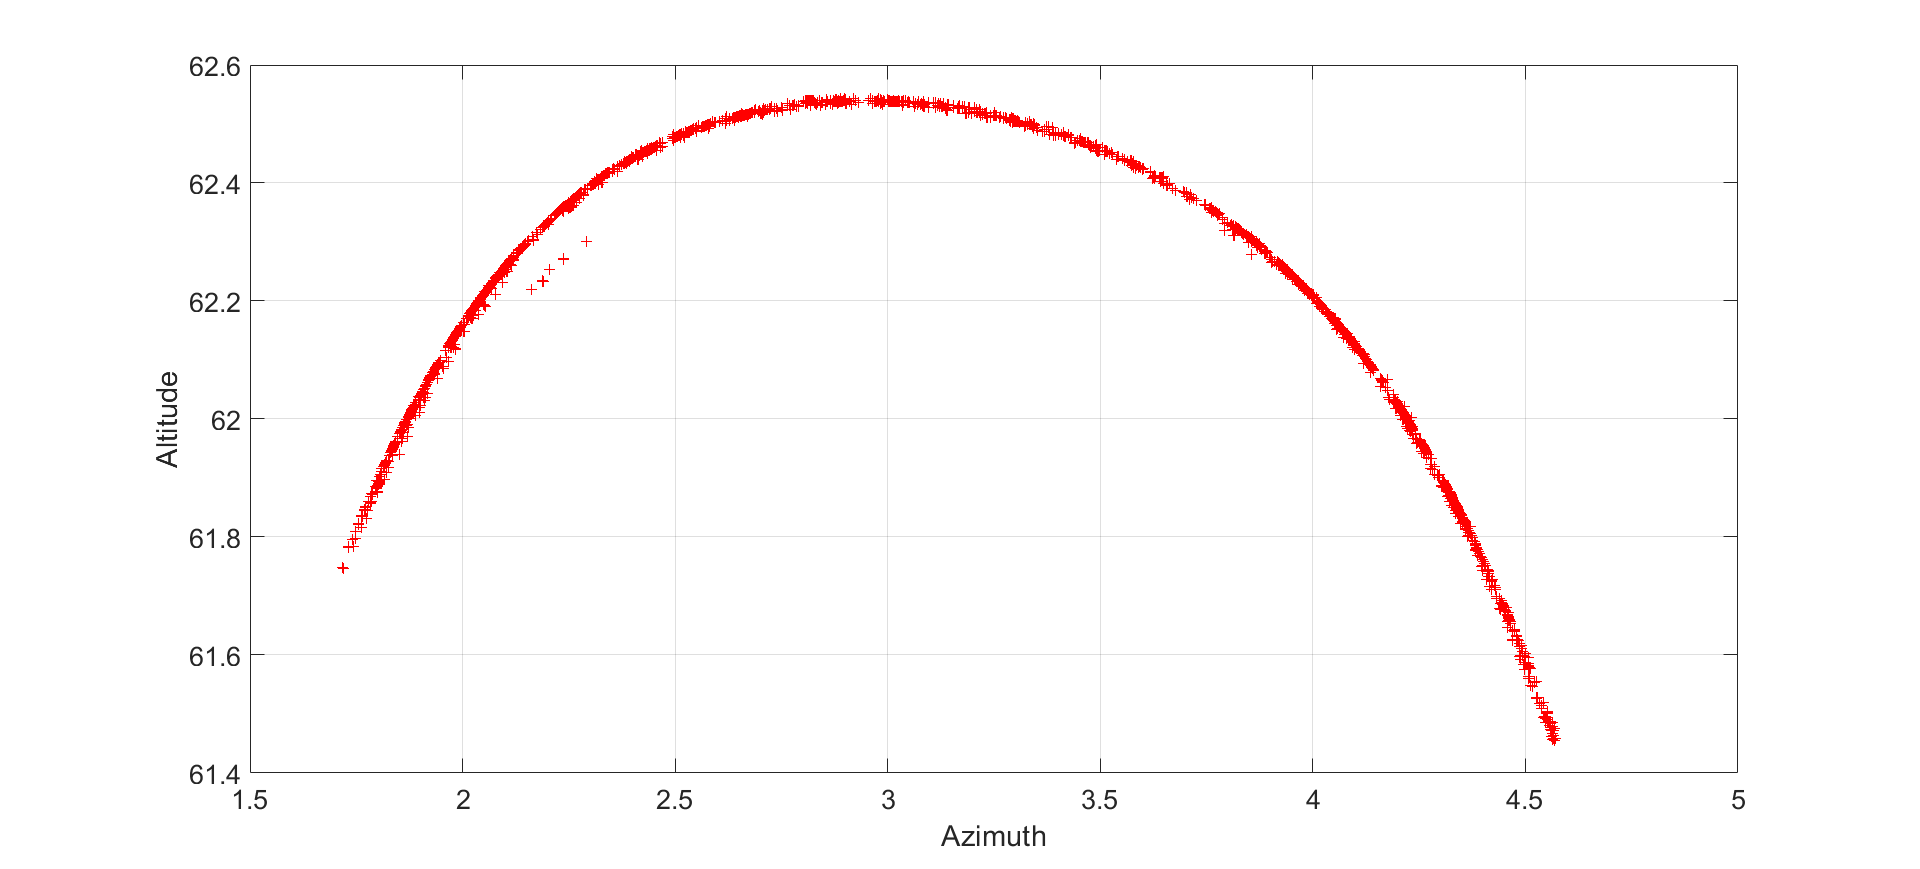
\includegraphics[width=0.9\textwidth]{AltvsAzHCS_11.png}
	\caption{Detections recorded by OGS in HCS (Tasking with Weightings)}\label{fig:}
\end{figure}

Figure~\ref{fig:AltvsAzHCS_comb} depicts the detections recorded by OGS in the horizontal coordinate system. The red crosses refer to the new detections recorded with the sensor tasking with weightings.\\


\begin{figure}[H]
	\centering
	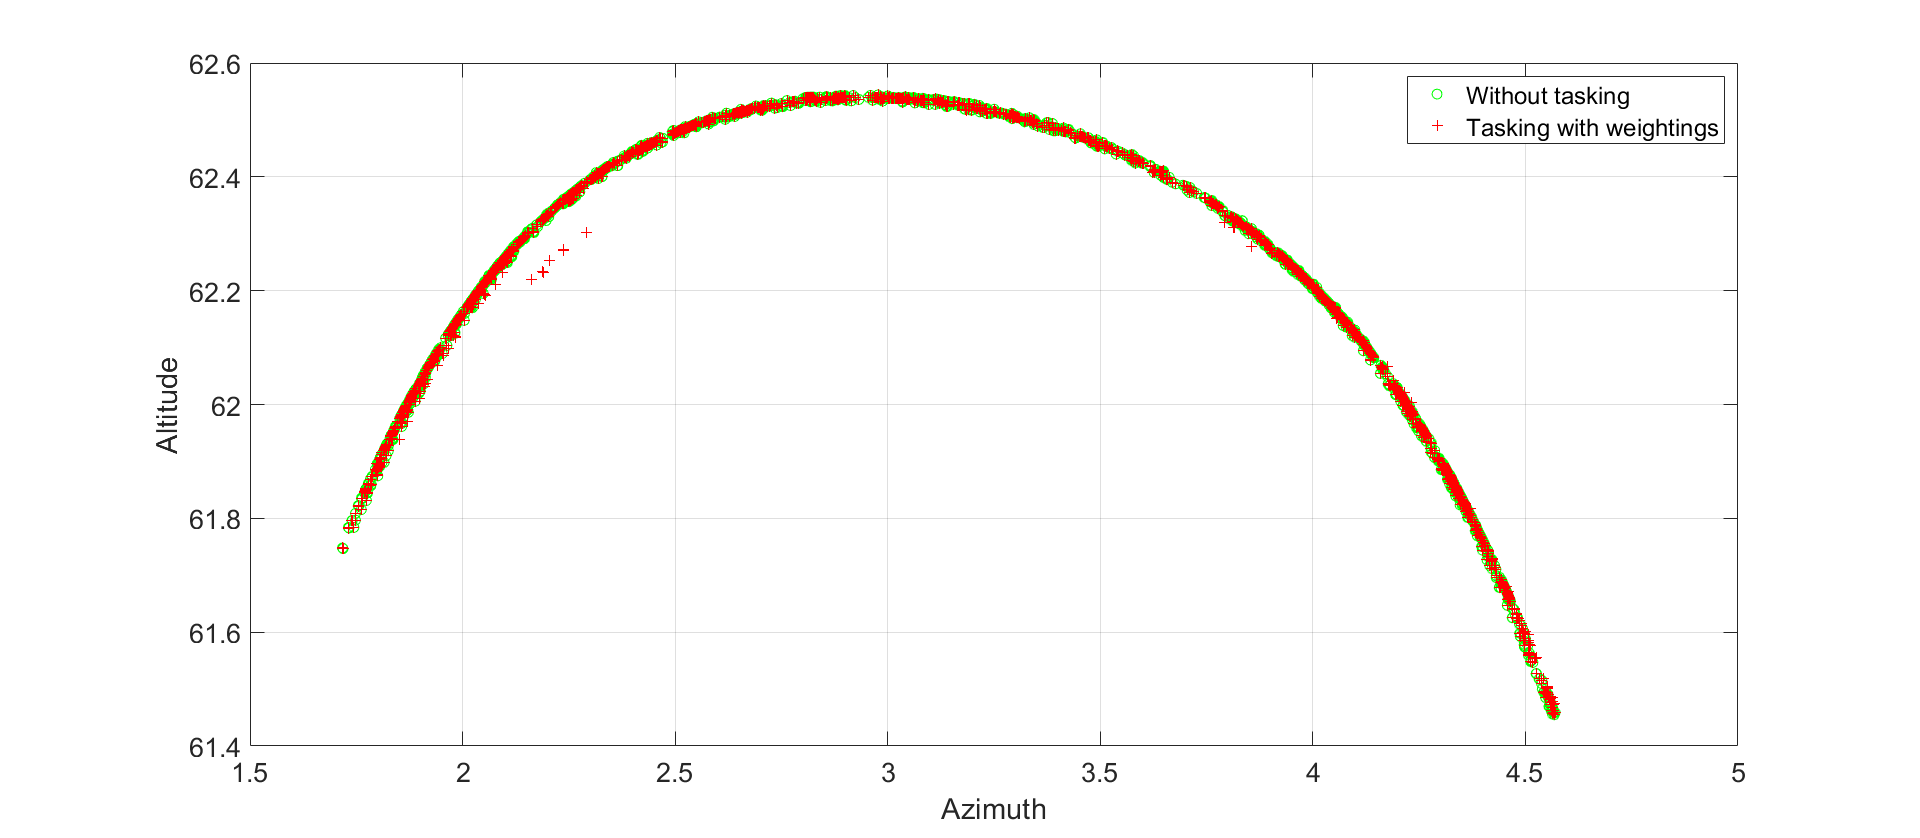
\includegraphics[width=0.95\textwidth]{AltvsAzHCS_comb.png}
	\caption{Detections recorded by OGS in HCS combined}\label{fig:AltvsAzHCS_comb}
\end{figure}


\begin{figure}[H]
	\centering
	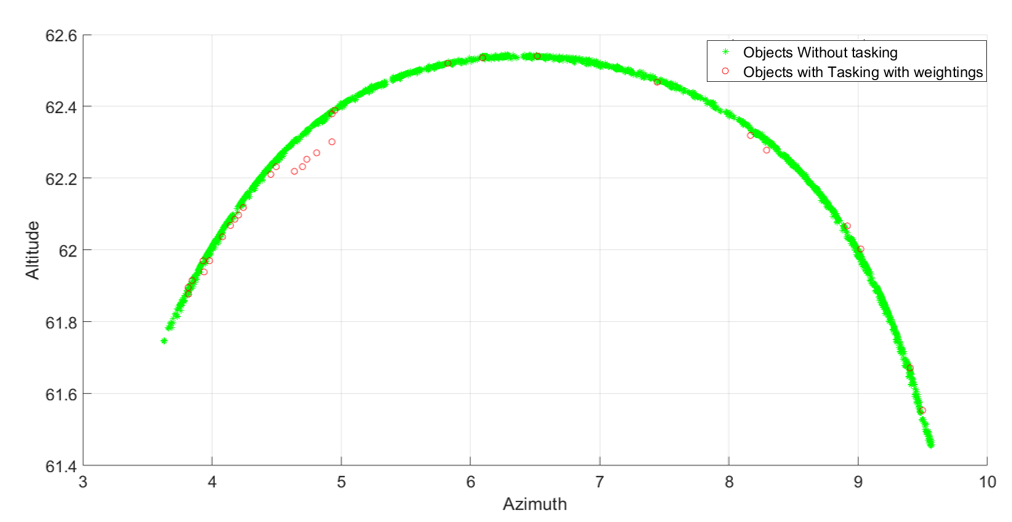
\includegraphics[width=0.95\textwidth]{AltvsAzObjects.png}
	\caption{Unique objects detected in the tasking with weightings}\label{fig:AltvsAzObjects}
\end{figure}

The employed algorithm utilized a simple stripe method for scanning the GEO vicinity, but its effectiveness in achieving an optimal search pattern is limited. Two key simplifications were introduced. Firstly, only fixed grid points in the right ascension and declination space were considered allowable viewing directions. The grid dimensions were determined by the field of view size of the sensor, ensuring comprehensive sky coverage without gaps. Improved search performance could be achieved if the spatial distribution of new targets were available, allowing the pointing direction to be set at the highest density of new targets.\\

The method's theoretical applicability extends to other orbital types besides GEO. However, careful consideration is required when designing search strategies for different orbits. Notably, a smaller grid size is sufficient for covering the GEO belt due to its dense distribution near the equator. Conversely, for different orbits like GTO and LEO, a larger field of regard might be necessary, posing challenges in discovering sparsely distributed new targets. The sensor-tasking performance is also contingent on catalog size, with surveying larger catalogs presenting computational complexities.\\

  \chapter{Zusammenfassung}

In der Zusammenfassung (mindestens 1,5 Seiten) sollen die theoretische Herleitung
und die wesentlichen Ergebnisse so aufgelistet werden, dass sie ohne Kenntnis der
vorherigen Abhandlung verständlich sind. Dabei wird in der Vergangenheit geschrieben und die wichtigsten Ergebnisse
der Arbeit wiedergegeben.
  \chapter{Fazit und Ausblick}

Ein kurzer Ausblick (max. ca. 1 Seite) kann dazu dienen, bei
Bearbeitung der gestellten Aufgabe entstandene neue Fragestellungen für zukünftige
Untersuchungen zu nennen.

  %===================================================
  %
  % Literaturverzeichnis
  %
  %---------------------------------------------------
  \addcontentsline{toc}{chapter}{Literaturverzeichnis}
    %\bibliographystyle{elsarticle-harv}
    \bibliographystyle{unsrtnat}
    \bibliography{literatur}
  
  %===================================================
  %
  % Abbildungsverzeichnis
  %
  %---------------------------------------------------
  \addcontentsline{toc}{chapter}{Abbildungsverzeichnis}
  \listoffigures
  \newpage
  
  %===================================================
  %
  % Tabellenverzeichnis
  %
  %---------------------------------------------------
  \addcontentsline{toc}{chapter}{Tabellenverzeichnis}
  \listoftables							% Tabellenverzeichnis
  \newpage
  
  %===================================================
  %
  % Symbol- und Abkürzungsverzeichnis
  %
  %---------------------------------------------------
  \chapter*{Symbolverzeichnis}						% Symbolverzeichnis
    \addcontentsline{toc}{chapter}{Symbolverzeichnis}			% fügt Symbolverzeichnis trotz * in das Inhaltsverzeichnis ein
          \printglossary[type=symbolslist, title=Symbole und Indizes]		% symbols
    \printglossary[type=acronymlist, title=Abk\"urzungen]		% abbreviations
 \glsaddall 
  %===================================================
  %
  % Anhang
  %
  %---------------------------------
  \begin{appendix}
    \chapter{Projektmanagement}
\label{cha:projekt}

\section{Work Breakdown Structure}
\label{sec:wbs}

\begin{landscape}
\begin{tikzpicture}[
  basic/.style   = {draw, text width=2.7cm, align=left, drop shadow, rectangle},
  root/.style    = {basic, text width=12cm, rounded corners=2pt, thin, align=center, fill=gray90},
  level 2/.style = {basic, rounded corners=2pt, thin, fill=gray80},
  level 3/.style = {basic, thin, fill=gray90, text width=2.6cm},
  level 1/.style={sibling distance=38mm}, edge from parent fork down, 
  edge from parent/.style={->,draw}, level distance=2.5cm,  >=latex]

% root of the the initial tree, level 1
\node[root] {\tb{Genauigkeit der Bahnbestimmung von Space Debris-Objekten mittels weltraumgest\"utzter optischer Sensoren}}
% The first level, as children of the initial tree
  child {node[level 2] (c1) {\tb{AP~1000} \\ Literatur-recherche}}
  child {node[level 2] (c2) {\tb{AP~2000} \\ Algorithmus-erstellung}}
  child {node[level 2] (c3) {\tb{AP~3000} \\ Implementie-rung \& Test}}
  child {node[level 2] (c4) {\tb{AP~4000} \\ Algorithmus-optimierung}}
  child {node[level 2] (c5) {\tb{AP~5000} \\ Simulation \\ $~~$}}
  child {node[level 2] (c6) {\tb{AP~6000} \\ Dokumentation \\ $~~$}};

% The second level, relatively positioned nodes
\begin{scope}[every node/.style={level 3}, node distance=6pt]
\node [below=of c1, xshift=10pt] (c11) {\tb{AP~1100} \\ Weltraumm\"ull-problematik};
\node [below=of c11] (c12) {\tb{AP~1200} \\ Beobachtung von Weltraum-m\"ull};
\node [below=of c12] (c13) {\tb{AP~1300} \\ Bahnbestim-mung mit optischen Sensoren};

\node [below=of c2, xshift=10pt] (c21) {\tb{AP~2100} \\ Aufbereitung von CCD-Daten in Winkelmessungen};
\node [below=of c21] (c22) {\tb{AP~2200} \\ Berechnung von Bahnparametern aus optischen Messungen};
\node [below=of c22] (c23) {\tb{AP~2300} \\ Hilfsalgorith-men};

\node [below=of c3, xshift=10pt] (c31) {\tb{AP~3100} \\ Einarbeitung in PROOF-Schnittstellen};
\node [below=of c31] (c32) {\tb{AP~3200} \\ Einbinden des Algorithmus als Unterroutine zu PROOF};
\node [below=of c32] (c33) {\tb{AP~3300} \\ Gesamttest};

\node [below=of c4, xshift=10pt] (c41) {\tb{AP~4100} \\ Verfeinerung der Aufarbeitung der CCD-Daten durch Subpixelinterpolation};
\node [below=of c41] (c42) {\tb{AP~4200} \\ Verbesserung der Bahnbestimmung durch Erh\"ohung der Anzahl von Objektsignalen};

\node [below=of c5, xshift=10pt] (c51) {\tb{AP~5100} \\ Simulation der Bahnbestimmung mit PROOF unter verschiedenen Randbedingungen};
\node [below=of c51] (c52) {\tb{AP~5200} \\ Feststellen der erzielbaren Genauigkeit der Bahnbestimmung};

\end{scope}

% lines from each level 1 node to every one of its "children"
\foreach \value in {1,2,3}
  \draw[->] (c1.212) |- (c1\value.west);

\foreach \value in {1,2,3}
  \draw[->] (c2.212) |- (c2\value.west);

\foreach \value in {1,2,3}
  \draw[->] (c3.212) |- (c3\value.west);

\foreach \value in {1,2}
  \draw[->] (c4.212) |- (c4\value.west);

\foreach \value in {1,2}
  \draw[->] (c5.212) |- (c5\value.west);
  
\end{tikzpicture}
\end{landscape}

\section{Zeitplan}
\label{sec:zeitplan}

\begin{landscape}
%\noindent\resizebox{\textwidth}{!}{	% Einfügen, falls zu groß
\begin{ganttchart}[hgrid,
                   time slot format = isodate, 
                   x unit=0.28cm,	% Zum komprimieren des Charts in x-Richtung
                   %y unit chart=0.7cm,
                   %compress calendar,	% Komprimiert den Chart in der Breite
                   calendar week text = {Woche~\currentweek},
                   chart element start border = right,
                   bar/.append style={fill=blue!40, rounded corners=2pt},
                   bar incomplete/.append style={fill=blue!10},
                   bar label node/.append style={align=left, text width=7cm},
                   group label node/.append style={align=left, text width=8cm},
                   milestone label node/.append style={align=left, text width=8cm},
                   bar progress label node/.style={right=2mm},
                   progress label text = {\pgfmathprintnumber[precision=0, verbatim]{#1}\%},
                  ]{2013-01-01}{2013-02-23}
  \gantttitlecalendar{year, month=shortname, week}\\
  %\gantttitle{2013}{59}\\
  \ganttgroup{AP 1000: Literaturrecherche}{2013-01-01}{2013-02-01}\\
  \ganttbar[progress=50]  {AP 1100: Weltraummüllproblematik}{2013-01-01}{2013-01-08}\\
  \ganttlinkedbar {AP 1200: Beobachtung von Weltraummüll}{2013-01-09}{2013-01-17}\\
  \ganttlinkedbar {AP 1300: Bahnbestimmung mit optischen Sensoren}{2013-01-17}{2013-02-01}\\
  %\ganttbar[progress=100]{AP 1300: TEXT}{2013-01-01}{2013-01-30}\\	% Beispiel für Fortschrittsbalken!
  
  \ganttgroup{AP 2000: Algorithmuserstellung}{2013-02-02}{2013-02-23}\\
  \ganttbar  {AP 2100: ...}{2013-02-02}{2013-02-09}\\
  \ganttbar  {AP 2200: ...}{2013-02-10}{2013-02-19}\\
  
  \ganttmilestone{Meilenstein}{2013-02-20}\\
  
 \end{ganttchart}
%}
\end{landscape}

\section{Work Package Description}
\label{sec:wpd}

\begin{table}[!h]
 \begin{center}
  \begin{tabular}{|p{35mm}||p{55mm}|p{50mm}||p{40mm}|}
   \hline
   \multicolumn{3}{|l||}{\textbf{}} & \multicolumn{1}{c|}{}\\
   \multicolumn{3}{|l||}{\textbf{}} & \multicolumn{1}{c|}{\textbf{AP 1100}}\\
   \multicolumn{3}{|l||}{\textbf{}} & \multicolumn{1}{c|}{}\\
   \hline\hline
   \textbf{Titel} & \multicolumn{2}{p{7cm}||}{\textbf{Genauigkeit der Bahnbestimmung von Space Debris-Objekten mittels weltraumgestützter optischer Sensoren}} 
& \textbf{Seite:} 1 von 1\\
   \hline
   \textbf{Verantwortlicher} & \multicolumn{2}{l||}{Sebastian Stabroth} & \textbf{Version:} 1.0\\
   \hline
   \multicolumn{3}{|l||}{} & \textbf{Datum:} 25.06.2003\\
   \hline\hline
   \textbf{Beginn} & \multicolumn{2}{l||}{T$_0$} & \\
   \hline
   \textbf{Ende} & \multicolumn{2}{l||}{T$_0$+1 Woche} & \textbf{Dauer}: 1 Woche\\
   \hline\hline
   \textbf{Bearbeiter} & \multicolumn{3}{l|}{Sebastian Stabroth}\\
   \hline\hline
   \multicolumn{4}{|p{150mm}|}{\textbf{Ziele:}}\\
   \multicolumn{4}{|p{150mm}|}{$\bullet$ Kenntnis über die Weltraummüllumgebung, Bahnbereiche von Space Debris-Populationen, Objektanzahlen und -größen}\\
   \multicolumn{4}{|p{150mm}|}{}\\
   \multicolumn{4}{|p{150mm}|}{\textbf{Input:}}\\
   \multicolumn{4}{|p{150mm}|}{$\bullet$ Literatur zum Thema Weltraummüll}\\
   \multicolumn{4}{|p{150mm}|}{}\\
   \multicolumn{4}{|p{150mm}|}{\textbf{Schnittstellen zu anderen APs:}}\\
   \multicolumn{4}{|p{150mm}|}{$\bullet$ \textbf{AP~5100} zur Simulation der Bahnbestimmung von Weltraummüll}\\
   \multicolumn{4}{|p{150mm}|}{}\\
   \multicolumn{4}{|p{150mm}|}{\textbf{Aufgaben:}}\\
   \multicolumn{4}{|p{150mm}|}{$\bullet$ Einlesen in die Thematik Weltraummüll}\\
   \multicolumn{4}{|p{150mm}|}{}\\
   \multicolumn{4}{|p{150mm}|}{\textbf{Ergebnisse:}}\\
   \multicolumn{4}{|p{150mm}|}{$\bullet$ Verständnis der Weltraummüllproblematik}\\
   \hline
  \end{tabular}
 \end{center}
\end{table}

\clearpage

\begin{table}[!h]
 \begin{center}
  \begin{tabular}{|p{35mm}||p{55mm}|p{50mm}||p{40mm}|}
   \hline
   \multicolumn{3}{|l||}{\textbf{}} & \multicolumn{1}{c|}{}\\
   \multicolumn{3}{|l||}{\textbf{}} & \multicolumn{1}{c|}{\textbf{AP 1200}}\\
   \multicolumn{3}{|l||}{\textbf{}} & \multicolumn{1}{c|}{}\\
   \hline\hline
   \textbf{Titel} & \multicolumn{2}{p{7cm}||}{\textbf{Titel des Arbeitspakets}} & \textbf{Seite:} X von Y\\
   \hline
   \textbf{Verantwortlicher} & \multicolumn{2}{l||}{Dein Name} & \textbf{Version:} 1.1\\
   \hline
   \multicolumn{3}{|l||}{} & \textbf{Datum:} DD.MM.YYYY\\
   \hline\hline
   \textbf{Beginn} & \multicolumn{2}{l||}{T$_0$} & \\
   \hline
   \textbf{Ende} & \multicolumn{2}{l||}{T$_0$+X Wochen} & \textbf{Dauer}: X Wochen\\
   \hline\hline
   \textbf{Bearbeiter} & \multicolumn{3}{l|}{Dein Name}\\
   \hline\hline
   \multicolumn{4}{|p{150mm}|}{\textbf{Ziele:}}\\
   \multicolumn{4}{|p{150mm}|}{$\bullet$ Ziel 1}\\
   \multicolumn{4}{|p{150mm}|}{$\bullet$ Ziel 2}\\
   \multicolumn{4}{|p{150mm}|}{$\bullet$ ...}\\
   \multicolumn{4}{|p{150mm}|}{}\\
   \multicolumn{4}{|p{150mm}|}{\textbf{Input:}}\\
   \multicolumn{4}{|p{150mm}|}{$\bullet$ Input 1}\\
   \multicolumn{4}{|p{150mm}|}{$\bullet$ ...}\\
   \multicolumn{4}{|p{150mm}|}{}\\
   \multicolumn{4}{|p{150mm}|}{\textbf{Schnittstellen zu anderen APs:}}\\
   \multicolumn{4}{|p{150mm}|}{$\bullet$ \textbf{AP XXXX} Beschreibung}\\
   \multicolumn{4}{|p{150mm}|}{$\bullet$ \textbf{AP ....} ...}\\
   \multicolumn{4}{|p{150mm}|}{}\\
   \multicolumn{4}{|p{150mm}|}{\textbf{Aufgaben:}}\\
   \multicolumn{4}{|p{150mm}|}{$\bullet$ Aufgabe 1}\\
   \multicolumn{4}{|p{150mm}|}{$\bullet$ ...}\\
   \multicolumn{4}{|p{150mm}|}{}\\
   \multicolumn{4}{|p{150mm}|}{\textbf{Ergebnisse:}}\\
   \multicolumn{4}{|p{150mm}|}{$\bullet$ Ergebnis 1}\\
   \multicolumn{4}{|p{150mm}|}{$\bullet$ ...}\\
   \hline
  \end{tabular}
 \end{center}
\end{table}
    %\include{WEITERER ANHANG}
  \end{appendix}

\end{document}
